\documentclass[12pt,a4paper,oneside,final,titlepage,openany,onecolumn]{book}
\usepackage[utf8]{inputenc}
\usepackage{graphicx}
\usepackage{changepage}
\usepackage [autostyle]{csquotes}
\usepackage[raggedright]{titlesec}
\MakeOuterQuote{"}
\usepackage{adjustbox}
\usepackage{float}
\usepackage{hyperref}
\hypersetup{colorlinks, linkcolor=black}
\newlength{\imgw}
\newlength{\imgh}
\setlength{\imgw}{\textwidth}
\setlength{\imgh}{5cm}
\newcommand{\image}[1]{\vspace{.5\baselineskip}\par\noindent\begin{adjustbox}{max width=\imgw, max height=\imgh, center}\includegraphics{#1}\end{adjustbox}\par\noindent}
\usepackage{caption}		% captionof
\usepackage{amsmath, mathtools}
\usepackage{makecell}		% makecell
\begin{document}

\author{notes by Giacomo Deodato}
\title{Clouds\\ \textbf{Distributed Systems\\and\\Cloud Computing}\\ - Prof. Pietro Michiardi -}
\date{Fall 2017}

\frontmatter
\maketitle
\tableofcontents
\mainmatter
\chapter{Scalable Algorithm Design}

\section{Introduction}
\par
What is big data? There are a lot of examples of vast repositories of data (the Web, Physics, Astronomy, Finance), their main characteristics are great \textbf{volume}, high growing \textbf{velocity} and \textbf{variety}.
\par\noindent
Generally, the bigger is the amount of data the smaller is the importance of the algorithm used. \textbf{With more data, accuracy of different algorithms converges}.
\par\noindent
The "Map Reduce" programming model is used to work with big data, it is a distributed programming model designed for large-scale data processing to run on clusters of commodity hardware.

\section{Key Principles}
\subsection*{Scale out instead of scale up}
For data intensive workloads, a large number of commodity servers is preferred over a small number of high-end servers.
I/O is very slow compared to processing speed therefore using more HDD in parallel instead of just one can improve performances. Moreover a sharing approach is better than shared nothing but sharing is difficult for various reasons (Synchronization, Deadlocks, Bandwidth).
\subsection*{Failures are the norm, not the exception}
Failures are mostly due to the scale and shared environment. There can be different types of failures (Permanent or Transient) coming from different sources (Hardware, Software, Cooling, Electrical).
\subsection*{Move processing to the data}
Generally, data intensive workloads are not processor demanding (no more HPC) so the \textbf{network becomes the bottleneck}. The framework exploits the \textbf{data locality principle} in order to assume processing and storage nodes to be collocated. \textbf{Distributed file systems} are necessary.
\subsection*{Process data sequentially, avoid random access}
Relevant datasets can be too large to fit in memory therefore \textbf{disk performance is a bottleneck} and systems are designed for batch processing involving mostly full scans of the data (organize computation in sequential reads).
\subsection*{Hide system-level details}
The framework abstracts away the distributed part of the system but in-depth knowledge of the framework is key.
\subsection*{Seamless scalability}
Scalability can be defined along two dimensions, in terms of \textbf{data}: given twice the amount of data, the same algorithm should take no more than twice as long to run; in terms of \textbf{resources}: given a cluster twice the size, the same algorithm should take no more than half as long to run.
The \textbf{embarrassingly parallel problem} aims at defining problems that require independent computation on fragments of the dataset.

\section{The Programming Model}
\subsection{Functional programming roots: Map and Fold}
Map and Fold are high order functions: functions that accept other functions as arguments.
\subsubsection{Map phase}
Given a list, Map takes as an argument a function \textit{f} (that takes a single argument) and applies it to all the elements in a list.
\subsubsection{Fold phase} 
Given a list, fold takes as arguments a function \textit{g} (that takes two arguments) and an initial value (an accumulator).The function is first applied to the initial value and the first item in the list, then the result is stored in an intermediate variable, which is used as an input together with the next item to a second application of g. The process is repeated until all items in the list have been consumed.
\newline\newline
Map can be seen as a transformation over a dataset. This transformation is defined by f. Each application to an element of the dataset happens in \textbf{isolation} so that the process can be parallelized.
\par
Fold can be seen as an aggregation operation defined by g. If we can group the elements of the list also this phase can proceed in parallel (remember about data locality).
\par
Associative and commutative operations allow performance gains through local aggregation and reordering.
\subsection{Hadoop MapReduce}
In Hadoop, Map corresponds to the map operations and Reduce to the fold one. The framework coordinates the two phases and aggregates (\textbf{group}) intermediate results in parallel.
\par
Key-Value pairs are the basic data structure. The programmer defines a mapper and a reducer as follows:
\[
\textit{map: (k1,v1) $\rightarrow$ [(k2, v2)] \qquad reduce: (k2, [v2]) $\rightarrow$ [(k3, v3)]}
\]
Between the map and reduce phases there is a parallel "group by" operation on intermediate keys. Intermediate data arrive at each reducer in order but there is no order across reducers. Intermediate keys are not stored on the distributed file system but on the local disk of each machine in the cluster.
\subsection{Example: word counter}
The mapper takes an input key-value pair, tokenizes the line and emits the intermediate key-value pairs: the word is the key and the integer is the value.
\par
The framework guarantees that all values associated with the same key are brought to the same reducer.
\par
The reducer receives all values associated to some keys, sums the value and writes the output key-value pairs: the key is the word and the value is the number of occurrences.
\subsection{Combiners}
Combiners are a general mechanism to reduce the amount of intermediate data and avoid huge network traffic (mini-reducers).
\par
Combiners are defined as follows:
\[
\textit{combiner: (k2, [v2]) $\rightarrow$ [(k2, v2)]}
\]
They have the same input as Reducers and the same output as Mappers.
\par
For commutative and associative operations Reducers code and Combiners code may be interchangeable but this is not true in the general case.
\begin{figure}[h!]
	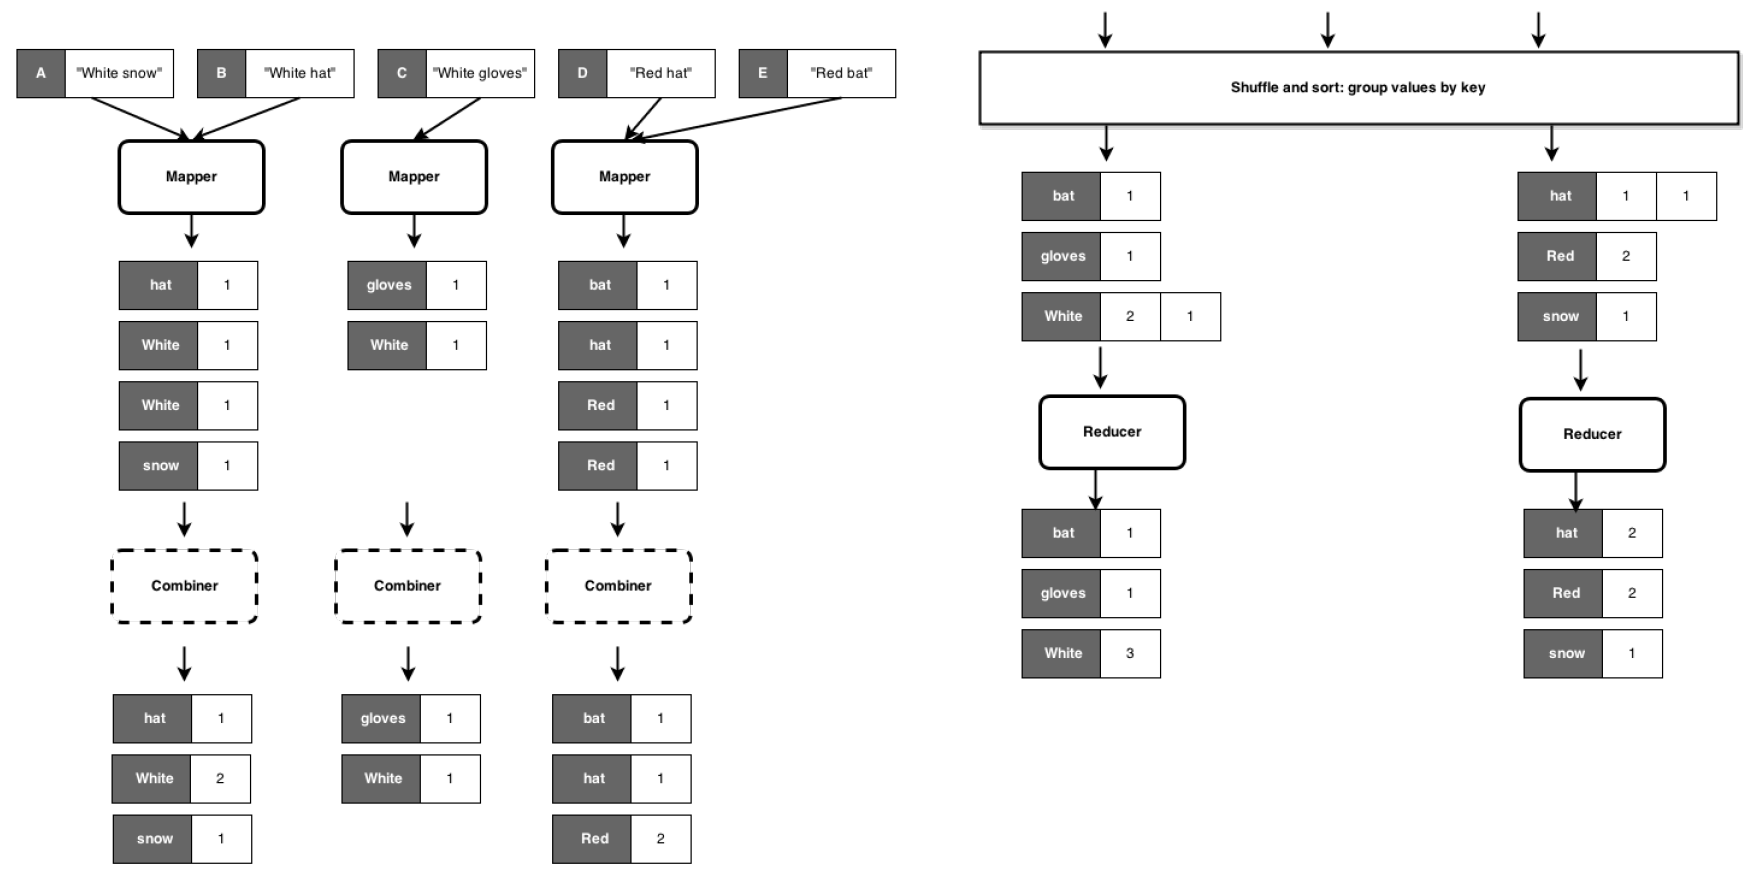
\includegraphics[width=\linewidth]{images/combiners.png}
	\caption{\textit{Word count using combiners.}}
\end{figure}
\subsection{Example: computing the mean}
We use an \textbf{identity mapper} which groups and sorts appropriately the input. Reducers keep track of the running sum and the number of integers encountered. The mean is emitted as the output of the reducer.
\par
The mean operation is not distributive hence a combiner cannot output partial means. 
\begin{figure}[h!]
	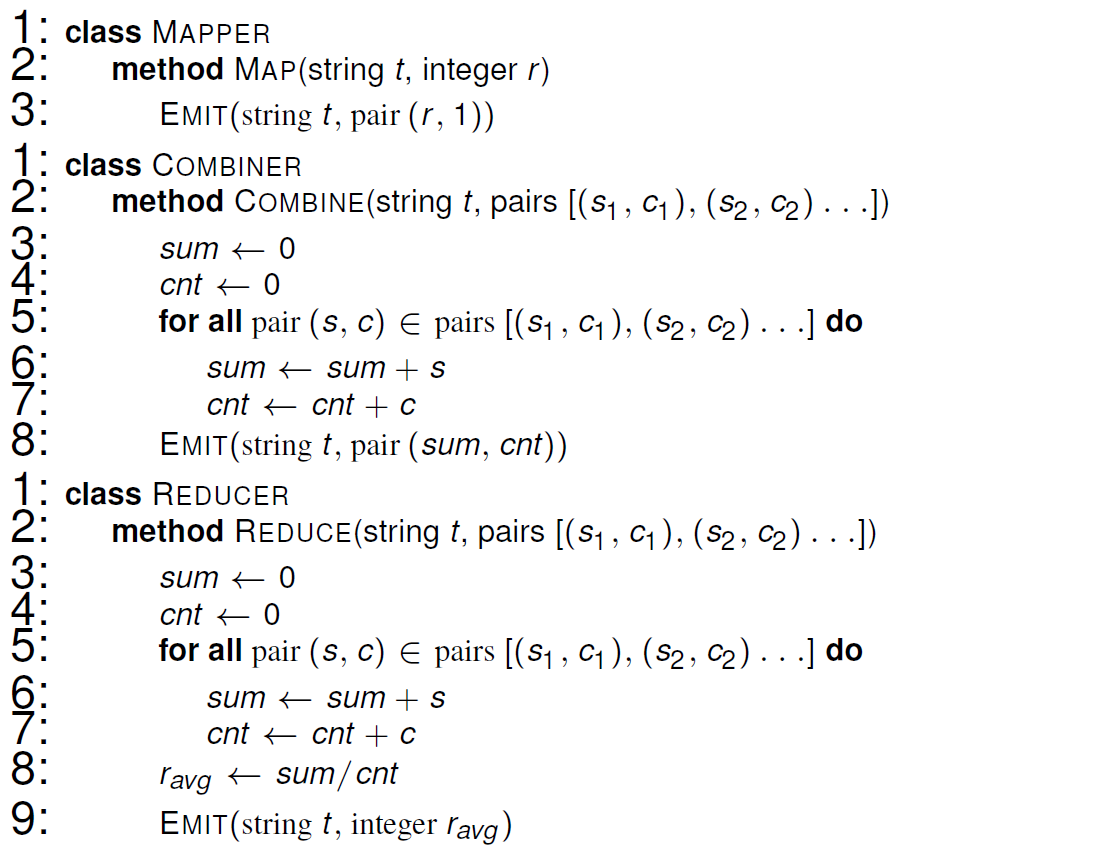
\includegraphics[width=\linewidth]{images/meanpseudocode.png}
	\caption{\textit{Pseudo-code to find the mean using combiners.}}
\end{figure}
%\captionof{figure}{pseudo code to find the mean}
\section {Basic Design Patterns}
\subsection{Algorithm design}
Developing algorithms involve preparing the input data, implementing the mapper and the reducer and, optionally, designing the combiner and the partitioner.
\par
Some of the aspects that can be controlled are: \textbf{the sort order} of intermediate keys (the order in which a reducer will encounter them) and \textbf{the partitioning of the key space} (the set of keys that will be encountered by a reducer). Moreover, the state can be preserved across multiple input and intermediate keys in mappers and reducers.
\par
Aspects that are not under the control of the designer are:
\begin{itemize}
	\item Where a mapper or a reducer will run;
	\item When a mapper or a reducer begins or finishes;
	\item Which key-value pairs are processed by a specific mapper or reducer;
\end{itemize}
\subsection{Local aggregation: In-Memory combiners}
In the context of data-intensive distributed processing, the most important aspect of synchronization is the \textbf{exchange of intermediate results} because network and disk latencies are expensive (Hadoop writes intermediate results to disk to be more fault tolerant). The use of combiners and preserving state across inputs reduces the number and size of key-value pairs to be shuffled.
\par
Combiners can be costly in terms of both CPU and I/O, \textbf{In-Mapper Combiners} could improve the performance by using an associative array (dictionary of key-value pairs) to cumulate intermediate results.
\par
To further improve the algorithm\footnote{A Java mapper object is created for each map task, the JVM reuse must be enabled.} the state can be preserved within and across calls to the map method by using \textbf{Initialize} (creates an across-map persistent data structure) and \textbf{Close} (emits intermediate key-value pairs only when all map tasks scheduled on one machine are done).
\begin{figure}[h!]
	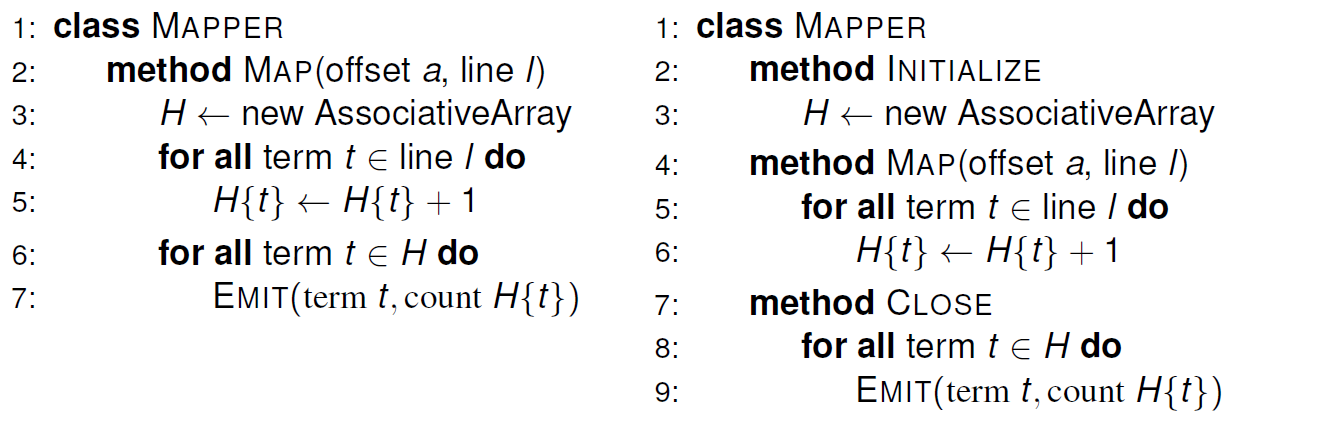
\includegraphics[width=\linewidth]{images/inmappercombiners.png}
	\caption{\textit{In-Memory combiners for the word count and mean problems.}}
\end{figure}
\par
In-Memory combiners are a \textbf{trade-off between memory usage and I/O}, the extent to which efficiency can be increased depends on the size of the intermediate key space. In-Memory combining breaks the functional programming paradigm due to state preservation, this implies that algorithm behaviour might depend on the execution order (works well with commutative/associative operations).
\par\noindent
Furthermore, it strictly depends on having enough memory to store intermediate results (possible solution: \textbf{block and flush}). Memory is an issue especially in hadoop because it is based on java and the JVM garbage collector doesn't always perform well.
\subsection{Pairs and stripes}
A common approach in MapReduce is to build complex keys (\textit{Pairs}) or values (\textit{Stripes}).
\subsubsection{Problem: Building word co-occurence matrices for large corpora}
The co-occurrence matrix is a square $n\times n$ matrix M. A cell $m _{ij}$ contains the number of times the word $w_i$ co-occurs with the word $w_j$ within a specific context (a sentence, a paragraph, a window of \textit{m} words).
\par\noindent
\textit{This matrix is useful to estimate the distribution of discrete joint events from a large number of observations.}
\par\noindent
The space requirement is $O(n^2)$ so the matrix could be bigger than the available memory (if the matrix is symmetric the space can be optimized).
\subsubsection{The pairs approach}
The mapper emits key-value pairs with \textbf{each co-occurring pair as the key} and the integer one (the count) as the value.
\par\noindent
The reducer receives pairs of co-occurring words (this \textbf{requires modifying the partitioner}) and computes the absolute count of the joint event. Then it emits the pair and the count (the cell of the matrix).
\subsubsection{The stripes approach}
The mapper stores co-occurrence information in an associative array, then it emits key-value pairs with words as keys and \textbf{the corresponding array as values}.
\par\noindent
The reducer receives all the arrays associated to the same word and performs an element-wise sum, then it emits the key-value pair in the form of word, associative array (the row of the matrix).
\begin{figure}[h!]
	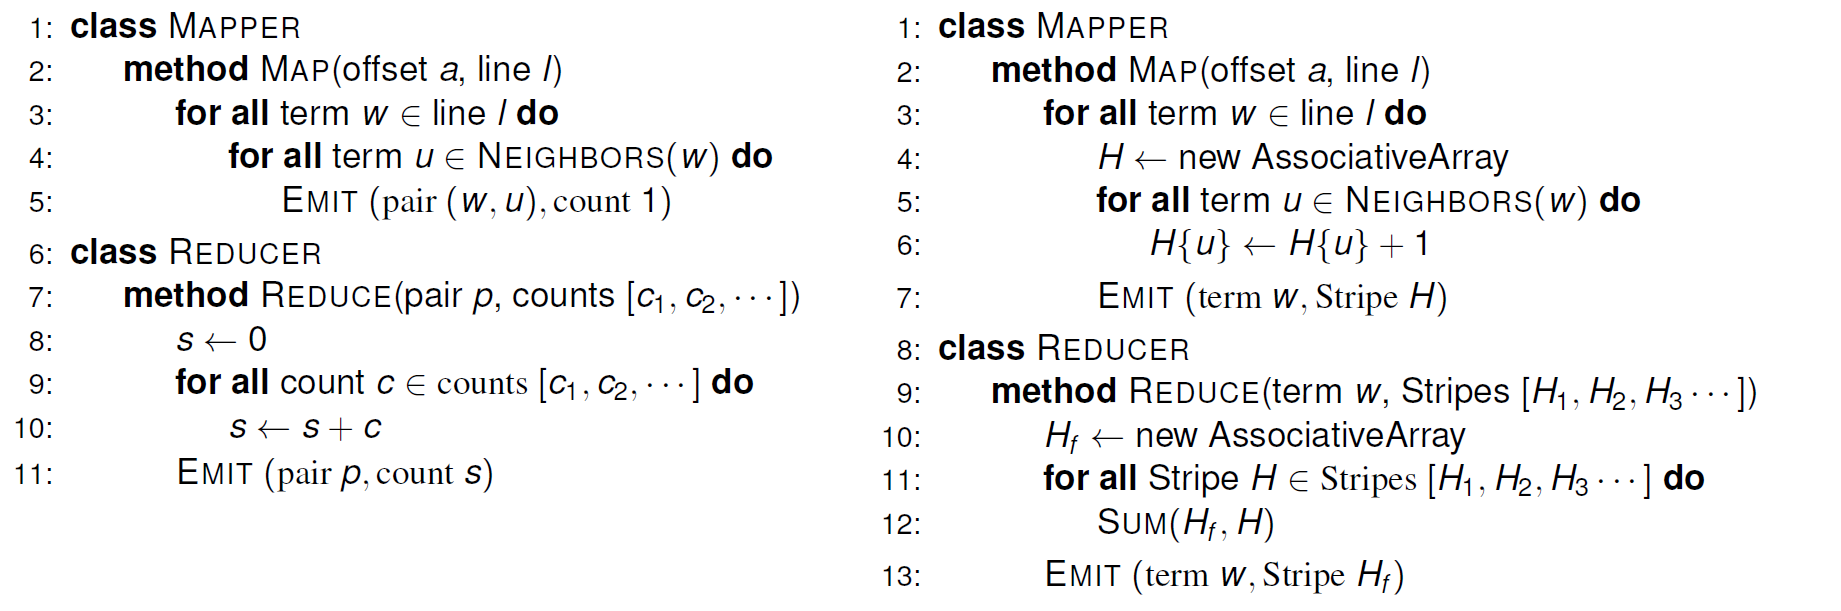
\includegraphics[width=\linewidth]{images/pairsandstripes.png}
	\caption{\textit{The pairs approach (left) and the stripes approach (right).}}
\end{figure}
\subsubsection{Pairs-stripes comparison}
Generally, the pairs approach generates a large number of key-value pairs over the network, \textbf{the benefit of combiners is limited} as it is less likely for a mapper to process multiple occurrences of a word. \textbf{It does not suffer of memory paging problems}.
\par\noindent
The stripes approach is more compact as it generates fewer intermediate keys but \textbf{the values have serialization/deserialization problems}. \textbf{It greatly benefits from combiners but may suffer of memory paging problems}.
\subsection{Order inversion}
\subsubsection{Problem: Building relative co-occurrence matrix}
The problem is similar as before but instead of absolut counts we need relative frequencies $f(w_j|w_i)$ because the word $w_i$ may co-occur frequently with word $w_j$ simply because one of the two is very common. Formally we compute:
\begin{equation*}
	f(w_j|w_i) = \dfrac{N(w_i, w_j)}{\sum_{w'}N(w_i, w')}
\end{equation*}
Where $N(\cdot,\cdot)$ is the number of times a co-occurring word pair is observed.
\newline
\par\noindent
With the stripes approach, in the reducer, the sum of all words that co-occur with $w_i$ (the denominator, \textit{marginal}) is available from the associative array.
\par
With the pairs approach we need to preserve the state in the reducer using a buffer in memory accumulating the count of all the words that co-occur with $w_i$.
\subsubsection{A basic approach}
We must \textbf{define the sort order of the pair} so that the keys are first sorted by the left word and then by the right word. In this way we can detect if all pairs associated with a word have been seen and use the in-memory buffer to compute the relative frequencies.
\par
We must \textbf{define an appropriate partitioner} so that all pairs with the same left word are sent to the same reducer. The default partitioner is based on the hash value of the intermediate key, modulus the number of reducers (for complex keys, the raw byte representation is used to compute the hash value).
\newline
\par
In order to implement this approach we need the to emit a special key-value pair $(w_i, *)$ to represent the marginal calculated by the combiner.
\par\noindent
The sort order of the intermediate key must be controlled so that the special key-value pair is processed first (define a custom partitioner).
\par\noindent
Preserve state (marginal) acrossmultiple keys in the reducer.
\par
The memory requirements are minimal because only the marginal (an integer) needs to be stored (no scalability bottleneck).

\chapter{Hadoop Internals}
	\subsubsection{Terminology}
	\par
		A \textbf{Job} is an execution of a mapper and reducer across a data set.
		\newline
		A \textbf{Task} is an execution of a mapper or a reducer on a slice of data.
		\newline
		A \textbf{Task Attempt} is an instance of an attempt to execute a task\footnote{Tasks attempt at least once, possibly more. Multiple crashes on input imply discarding it. Multiple attempts may occur in parallel (speculative execution), the TaskID is not a unique identifier.}.
\section{Hadoop Distributed File System}
	\subsection{Motivations}
	\par
		As dataset size increase, more computing capacity is required for processing and, as computing capacity grows, the link between the computing nodes and the storage nodes becomes a bottleneck.
		\newline
		Special-purpose interconnections for high performance computing are a costly solution, a distributed file system is not mandatory but highly desirable.
		\newline
	\par
		The key idea is to abandon the separation between compute and storage nodes: \textbf{large datasets are partitioned across a number of separate (commodity) machines} in a network-based system with all its complications (failure tolerance).
		\newline
		Distributes file systems for MapReduce are built upon previous results with different requirements: \textbf{write once, read many workloads} (do not handle concurrency but allow replication). They are optimized for throughput, not for latency.
	\subsection{Blocks}
	\par
		Files are broken into big [64, 128] MB block-sized chunks\footnote{Files smaller than a single block do not occupy a full block's worth of underlying storage.} to \textbf{make transfer times larger than seek latency}, this also avoids problems related to metadata management.
	\par
		Blocks are stored on independent machines and replicated across the local disks of nodes in the cluster (reliability and parallel access), replication is handled by storage nodes themselves.
	\subsection{Architecture}
		\par\indent
		\par\indent\textbf{Namenode}: Keeps metadata in RAM (150 bytes for each block). Persistence of metadata depends on synchronous and atomic writes to NFS. Maintains overall \textbf{health} of the file system.
		\par
		\textbf{Secondary NodeName}: It merges the namespace with the edit log. To recover from a failure of a NameNode, use the NFS copy of metadata and switch the secondary to primary.
		\par
		\textbf{DataNode}: They store data and talk to clients. They report periodically to the NameNode the list of blocks the hold.
		\begin{figure}[h!]
			\centering
			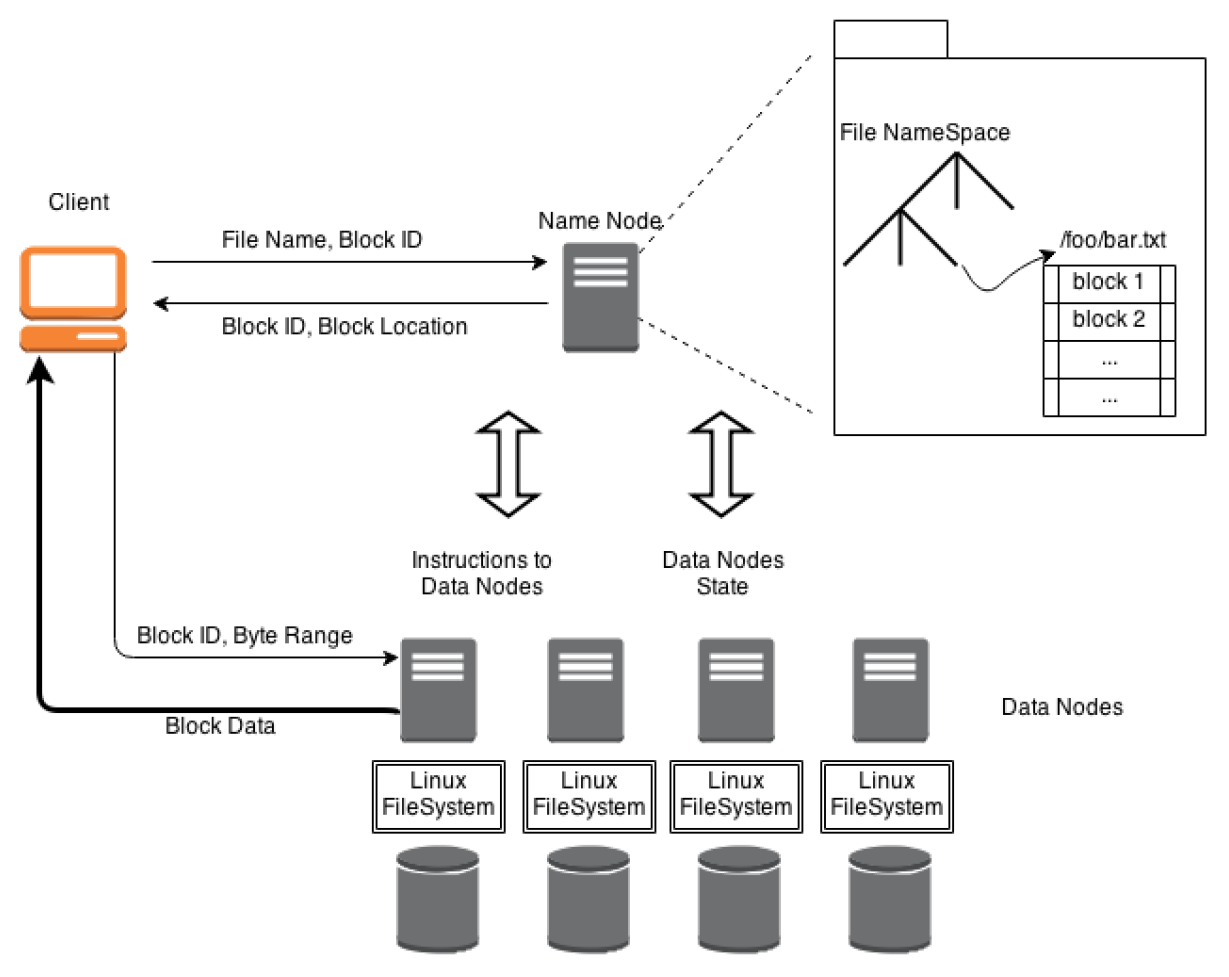
\includegraphics[width=0.8\linewidth]{images/arch_sketch.png}
			\caption{\textit{Architecture sketch of HDFS operations.}}
		\end{figure}
	\subsubsection{File read}
		\par
		The NameNode is only used to get the block location. Unresponsive DataNodes are discarded by clients.
		\newline
		To external clients, for each block, the namenode returne a set of datanodes sorted according to their proximity to the client.
		\newline
		To MapReduce clients, TaskTracker and DataNodes are collocated and, for each block, the namenode usually returns the local DataNode.
	\subsubsection{File write}
		\par
		The client asks the NameNode for a list of suitable DataNodes, the list forms a pipeline: the first DataNode stores a copy of a block, then forwards it to the second, and so on (\textbf{replication}).
		\newline
		The \textbf{replica placement is a trade-off between reliability and bandwidth}, the default placement requires a copy on the same node of the client, a replica \textbf{off-rack} and another on the same rack as the second but on a different node.
	\subsubsection{HDFS coherency model}
		\par
		The namespace is updates but the block contents may not be visible after a write is finished. To force synchronization it is necessary to use \textit{sync()}, but it involves some overhead (trade-off between robustness/consistency and throughput).
		\newline
		Multiple writers for the same block are not supported but different block can be written in parallel by using MapReduce.

\section[Hadhoop MapReduce]{Hadhoop MapReduce\protect\footnotemark}
\footnotetext{MapReduce APIs are evolving fast, therefore it is advised to use the appropriate API documentation and Eclipse instead of the prof notes.}
	\subsection{Anatomy of a job run}
		\begin{figure}[h!]
			\centering
			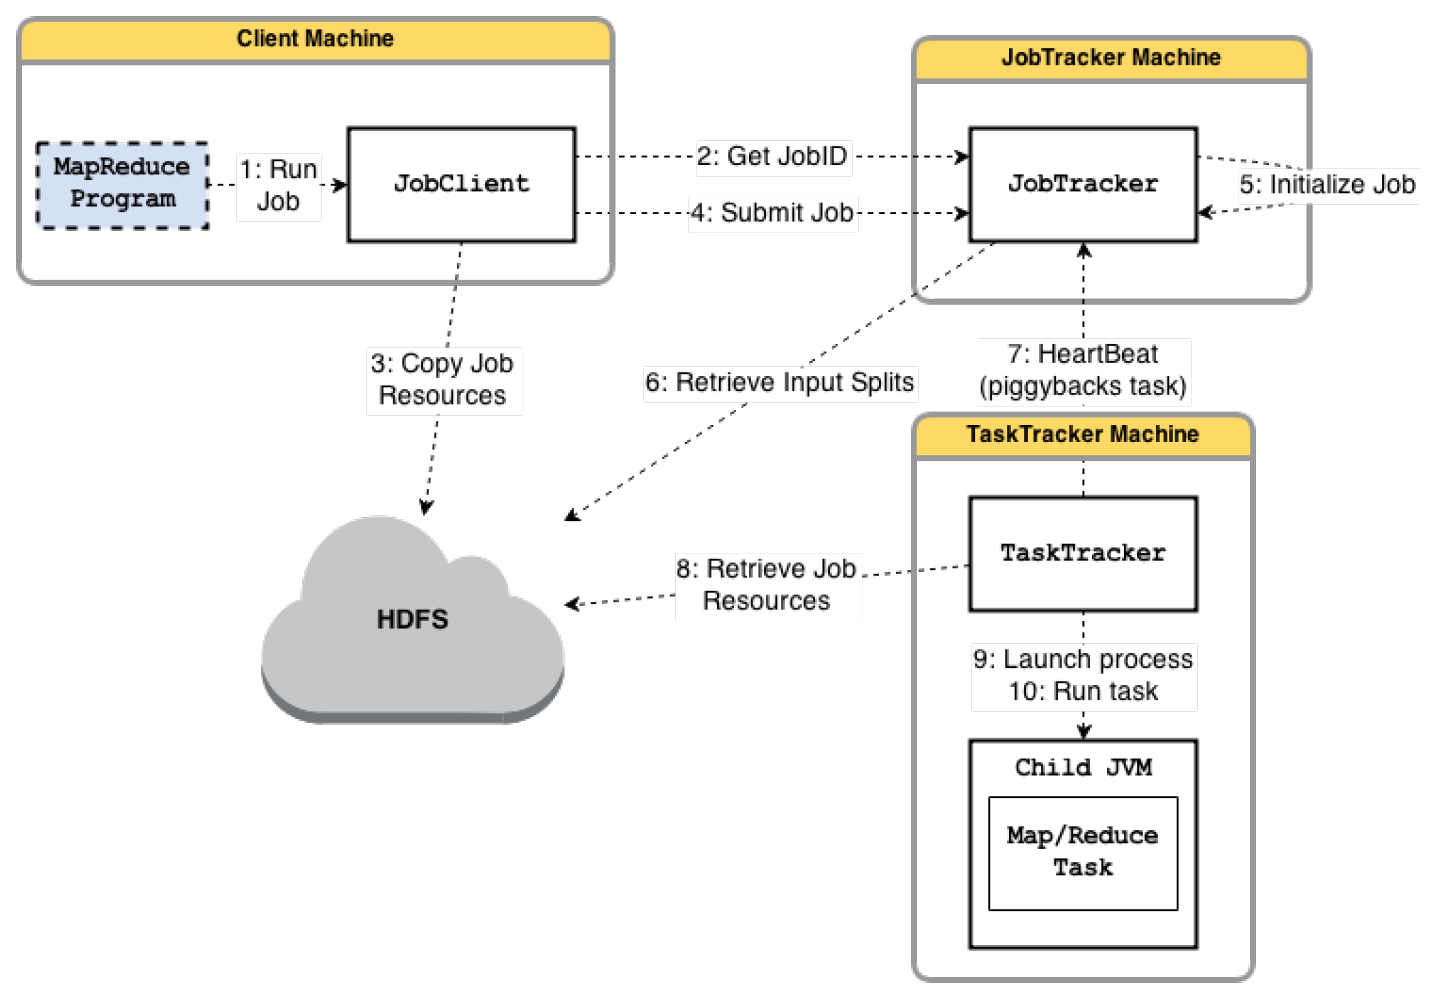
\includegraphics[width=\linewidth]{images/jobrun.png}
			\caption{\textit{Anatomy of a MapReduce job run.}}
		\end{figure}
	\subsubsection{Job submission}
		\par
		The \textit{runJob()} method creates a new instance of a \textbf{JobClient}, then it calls \textit{submitJob()} on this class.
		\newline
		Some simple verifications are done on the job to check if there is an output directory, input splits, and if the JAR of the job can be copied to the HDFS\footnote{The JAR of the job is replicated 10 times}.
	\subsubsection{Job initialization}
		\par
		The \textbf{JobTracker} is responsible for the creation of an object for the job. It encapsulates its tasks and does the \textbf{bookkeeping} with the tasks' status and progress.
		\newline
		It performs scheduling by maintaining a queue\footnote{Queuing disciplines are pluggable.}.
		\newline
		The JobTracker retrieves input splits (computed by JobClient) and determines the number of Mappers based on their number, then it reads the configuration file to set the number of reducers.
	\subsection{Scheduling}
		\subsubsection{Task assignment}
			\par
			The TaskTrackers periodically send \textbf{heartbeats} to the JobTracker. Heartbeats contain information on availability of the TaskTracker to execute a task. The JobTracker piggybacks a task if the TaskTracker is available.
			\newline
			The JobTracker first needs to select a job (\textit{job scheduling}). TaskTrackers have a fixed number of slot for map and reduce tasks, \textbf{the JobTracker gives priority to the map tasks}.
			\newline
			\textbf{The JobTracker is topology aware}, this is useful for map tasks (data locality) but not for reduce tasks (shuffle, it does not know which reducer will have which data).
		\subsubsection{Task execution}
			\par
			After the assignment is done the TaskTracker copies the JAR from the HDFS, creates a local working directory and creates an instance of TaskRunner.
			\newline
			TaskRunner launches a child JVM (prevents bugs from stalling the TaskTracker). A new child JVM is created for InputSplit (can be overriden with JVM Reuse, in-memory combiners).
			\newline
		\par\noindent
		Some examples of scheduler are: FIFO scheduler, Fair scheduler (every user gets a fair share of the cluster capacity over time) and Capacity Scheduler (hierarchical queues with FIFO scheduling in each queue).
	\subsection{Handling failures}
		\subsubsection{Task failure}
			\par
			If a map or reduce task throws a \textbf{runtime exception} then the child JVM reports back to the TaskTracker, the TaskTracker logs the error, marks the task attempt as failed and frees a slot to run another task.
			\newline
			If there is a \textbf{hanging task}, the TaskTracker notices no progree updates (timeout) and kills the child JVM.
			\newline
			The JobTracker is notified of a failed task, it avoids rescheduling the task on the same TaskTracker, if a task fails 4 times, it is not rescheduled and the job fails.
		\subsubsection{TaskTracker failure}
			\par
			If a TaskTracker fails (crash or slow), heartbeats are not sent to the JobTracker and, after a timeout, the latter will remove the TaskTracker from his scheduling pool (may blacklist a TaskTracker if too many tasks fail).
			\newline
			The JobTracker needs to reschedule all the tasks (even completed and in progress ones).
		\subsubsection{JobTracker failure}
			\par
			Currently, Hadoop has no mechanism for this kind of failure (future/commercial releases: multiple JobTrackers, ZooKeeper, High Availability).
		\subsection{Shuffle and sort: Map side}
			\par
			The MapReduce framework guarantees the input to every reducer to be sorted by key, the process by which the system sorts and transfers map outputs to reducers is known as shuffle.
			\newline
			Shuffle is the most important part of the framework, a good understanding allows optimizing both the framework and the execution time of MapReduce jobs.
			\begin{figure}[h!]
				\centering
				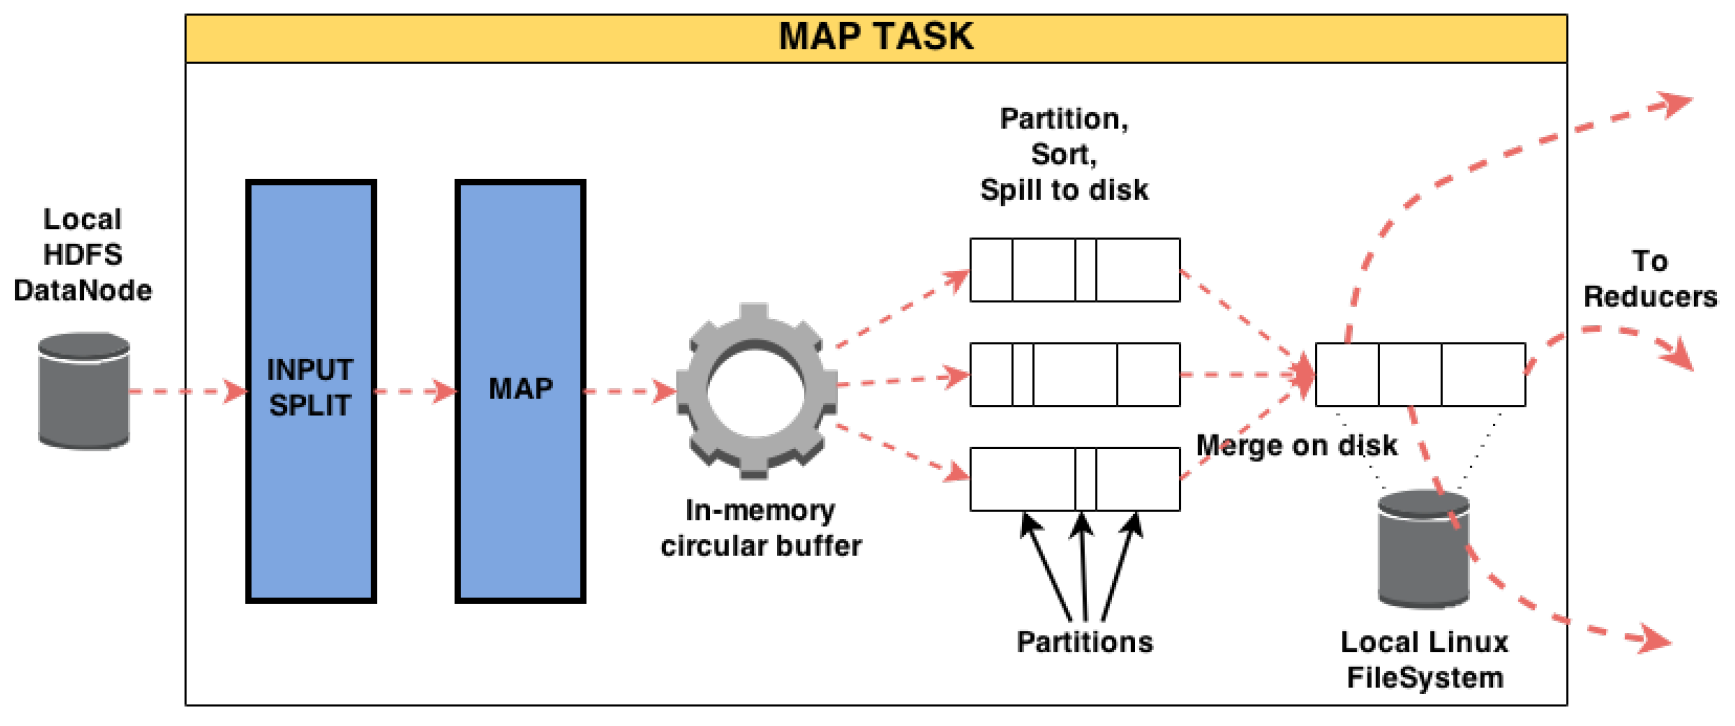
\includegraphics[width=\linewidth]{images/sasmapside.png}
				\caption{\textit{Shuffle and sort: the Map side.}}
			\end{figure}
			\par
			The output of a map task is not simply written to disk, it passes from a circular memory buffer. The buffer has a threshold based mechanism to \textbf{spill} buffer content to disk. The map output is written to the buffer while spilling on disk, if the buffer fills up while spilling the map task is blocked.
			\newline
			The disk spills are written in round-robin to a local directory. The output data are partitioned corresponding to the reducers they will be sent to, within ieach partition, data is \textbf{sorted in memory}.
			\newline
			Optionally, if there is a combiner, it is executed just after the sort phase.
			\newline
			Once the map task finishes there are many spills, such spills are merged into a single, partitioned, and sorted out file.
		\subsection{Shuffle and sort: Reduce side}
			\par
			The map output file is located on the local disk of a TaskTracker. Another TaskTracker (in charge of a reduce task) requires input from many other TaskTracker (that finished their map tasks).
			\newline
			When a map task finishes, it notifies the parent TaskTracker. The parent TaskTracker notifies (heartbeat) the JobTracker. A thread in the reducer polls periodically the JobTracker. TaskTrackers do not delete local map output as soon as a reduce task has fetched them (reliability).
			\begin{figure}[h!]
				\centering
				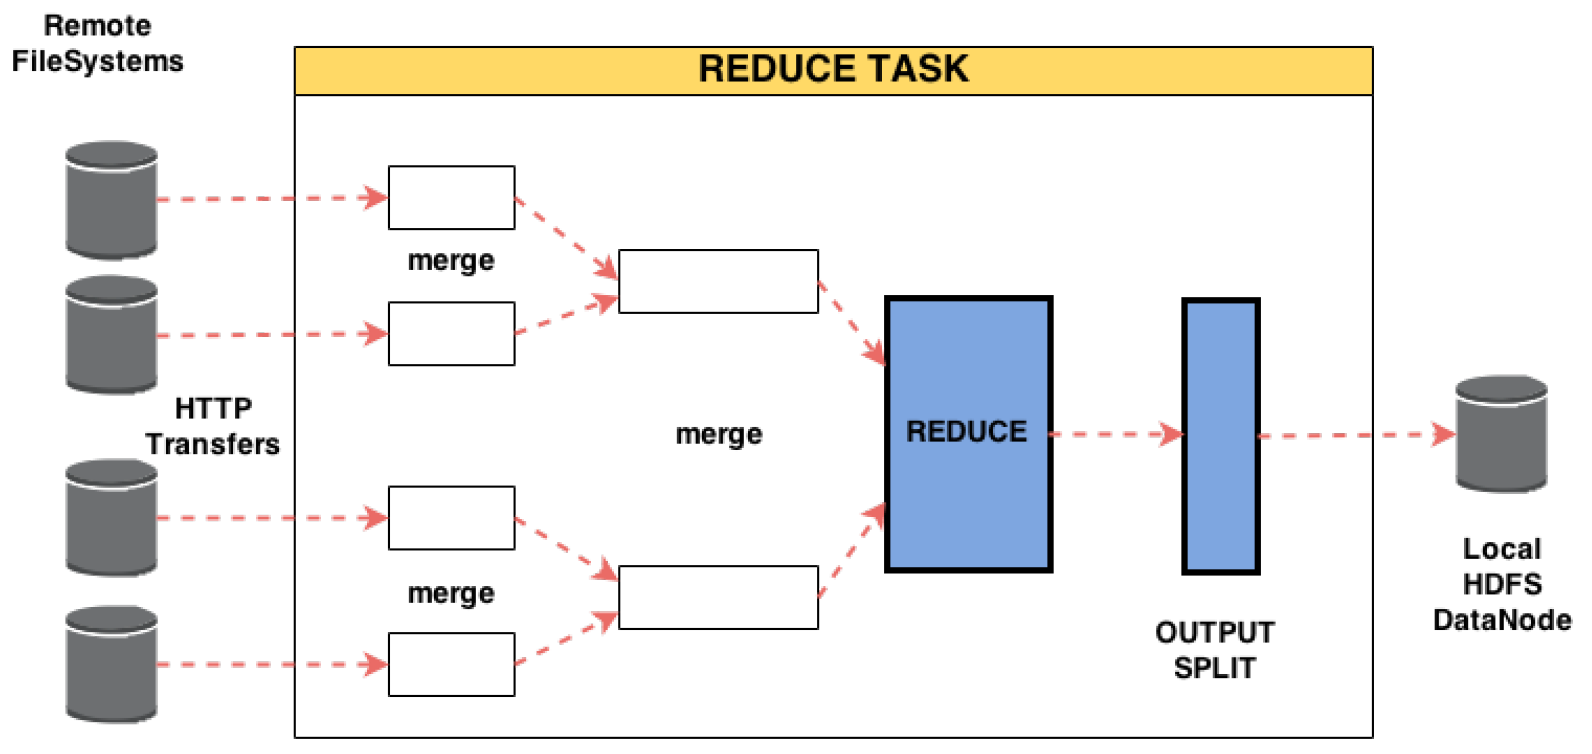
\includegraphics[width=\linewidth]{images/sasreduceside.png}
				\caption{\textit{Shuffle and sort: the Reduce side.}}
			\end{figure}
			\par
			There is a small number of copy threads that can fetch map outputs in parallel. The map output is copied to the TaskTracker running the reducer \textbf{in memory} (if they fit, otherwise they are copied on disk).
			\newline
			A background thread merges all partial inputs into larger, \textbf{sorted} files.
\chapter{Apache Spark Internals}

\section{Introduction and Motivations}
	\par
	From a \textbf{software engineering} point of view the Hadoop \textbf{code base} is huge (while Spark's is smaller) and contributions/extensions are cumbersome.
	\newline
	\par\noindent
	From a \textbf{system/framework} point of view Spark is better because of its \textbf{unified pipeline}:
	\begin{itemize}
		\item Spark Streaming for stream processing
		\item GraphX for graph processing
		\item MLLib, Machine Learning Library
		\item Spark SQL for SQL on Spark
	\end{itemize}
	And its simplified data flow and faster processing speed (Spark is faster not only because of the simplified data flow, but also because it \textbf{avoid materializing data on HDFS} after each iteration).
	\newline
	\par\noindent
	From a \textbf{data abstraction} point of view Spark introduces a new fundamental abstraction: the \textbf{RDDs}. They are easy to extend with new operators and there is a more descriptive computing model. Computation is organized in multiple stages: \textbf{Transformations} apply user code to distributed data in parallel while \textbf{Actions} assemble final output of an algorithm, from distributed data.
\section{Anatomy of a Spark Application}
	\par
	\begin{figure}[H]
		\centering
		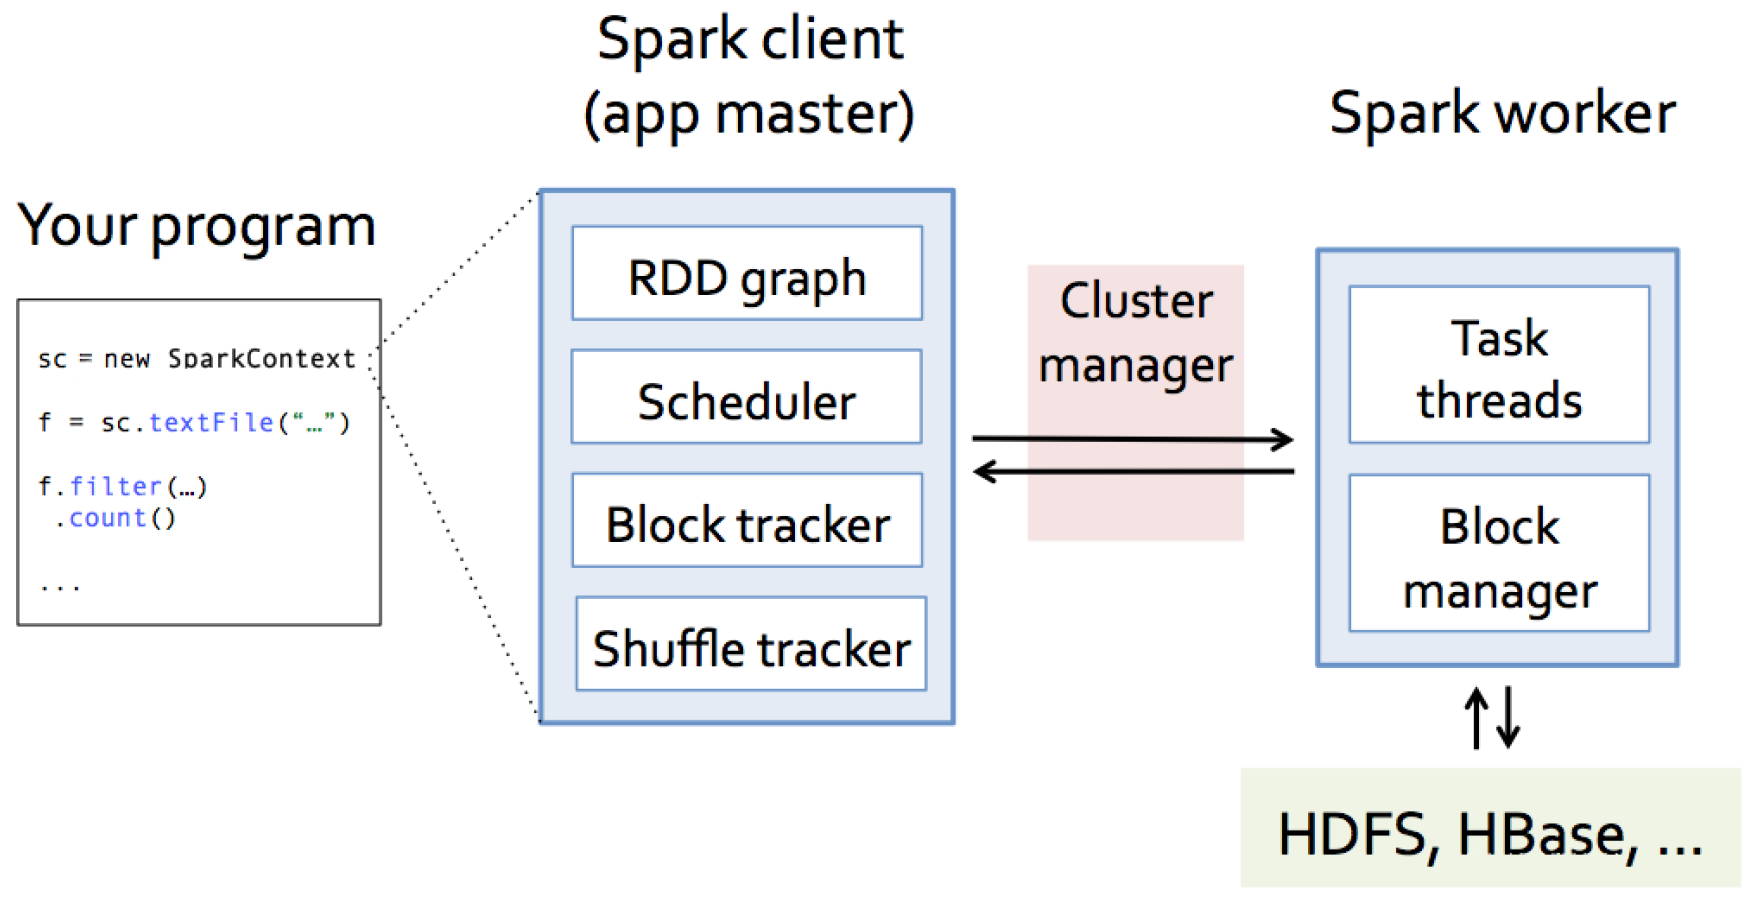
\includegraphics[width=\linewidth]{images/sparkcomp.png}
		\caption{\textit{Spark components details.}}
	\end{figure}
	Spark applications respect the same locality principle as Hadoop and use caching for filtered RDDs.
	\newline
	A generic application creates a \textbf{SparkContext} which is a core component of the \textbf{DriverProgram}, then it registers to the \textbf{ClusterManager}. Upon an action, the driver program submits the job to the cluster manager.
	\newline
	The \textbf{Cluster Manager} does not know about stages, it starts executors on workers nodes.
	\newline
	The \textbf{RDD objects} build the operator for the Directed Acyclic Graph (\textbf{DAG}).
	\newline
	The \textbf{DAG Scheduler} splits the DAG into stages of tasks (	lazy evaluation model) and submits each stage and its task as they are ready to the task scheduler, it uses a listener for the results.
	\newline
	The \textbf{Task Scheduler} launch tasks on \textit{executors} via Master and retries failed and straggler tasks, it reports to the DAG scheduler.
	\newline
	The \textbf{Worker} launches spark executor in a process, tasks are launched in separate threads, one per each core on the worker node.
	\begin{figure}[H]
		\centering
		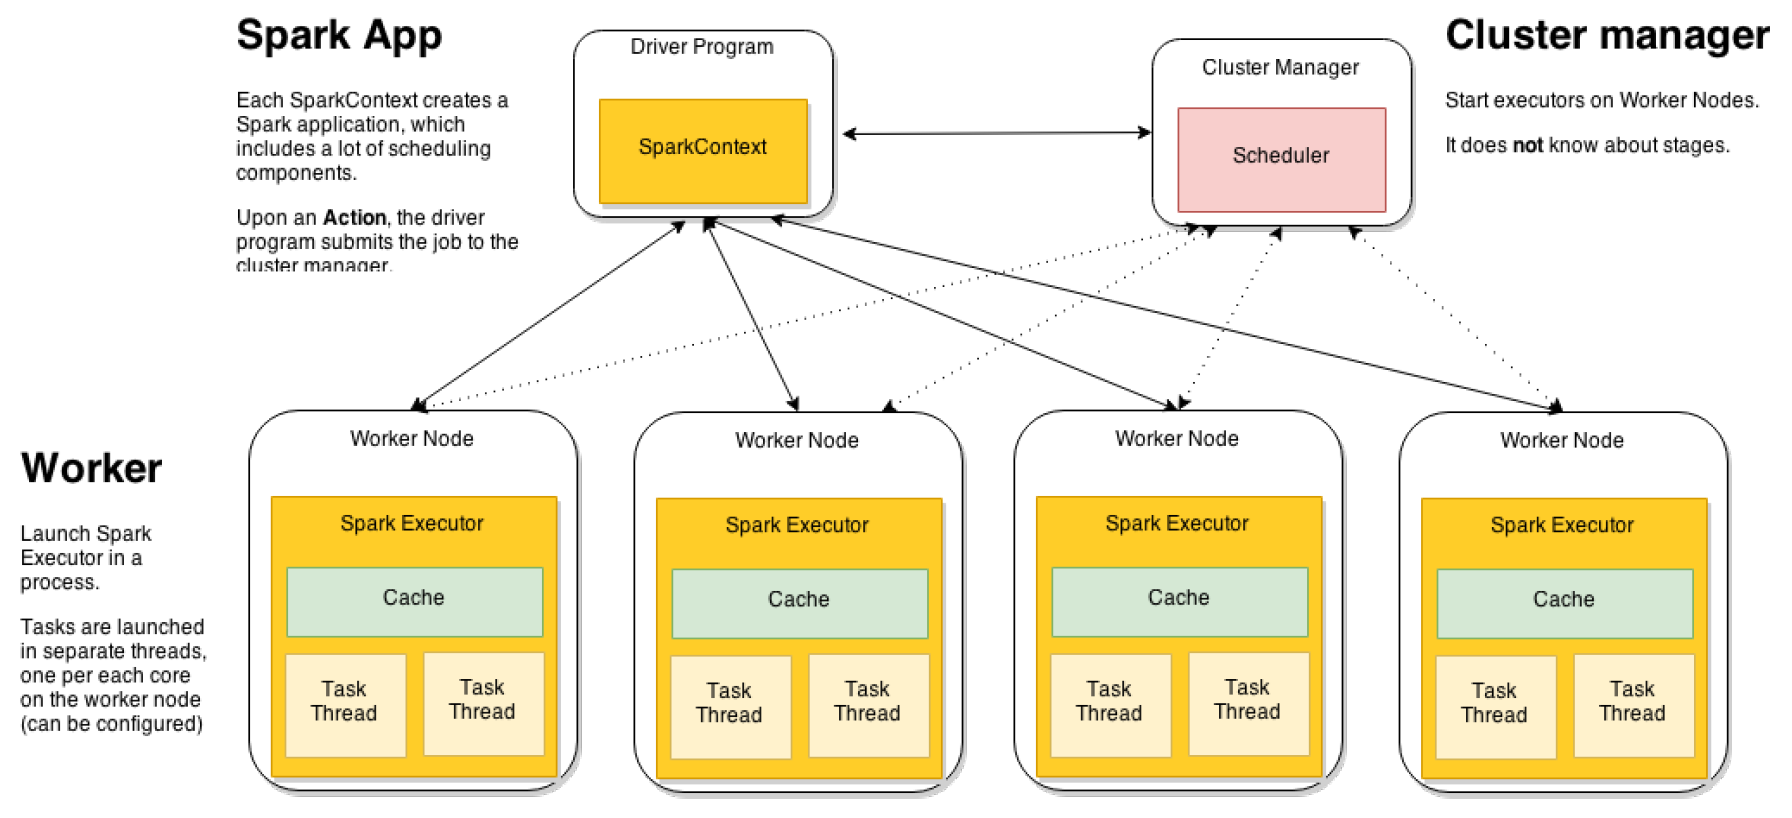
\includegraphics[width=\linewidth]{images/sparkcompsys.png}
		\caption{\textit{Spark components: system level view.}}
	\end{figure}
\section{Spark Deployments}
	\par
	The general workflow of a Spark application is the following:
	\begin{enumerate}
		\item The Spark application creates a \textbf{SparkContext}, which initializes the \textbf{DriverProgram}
		\item It registers to the \textbf{ClusterManager}
		\item It asks resources to allocate executors
		\item It schedules Task execution
	\end{enumerate}
	The master node is the machine running the Master program and the Driver (SparkContext and application code).
	\newline
	The worker nodes are machines that run executors. They host one or multiple Workers with one JVM (1 UNIX process) per each one. Each Worker can spawn one or more Executors.
	\newline
	The Executors run tasks. They run in child JVM (1 UNIX process) and execute the tasks using threads in a \textit{ThreadPool}
	\begin{figure}[H]
		\centering
		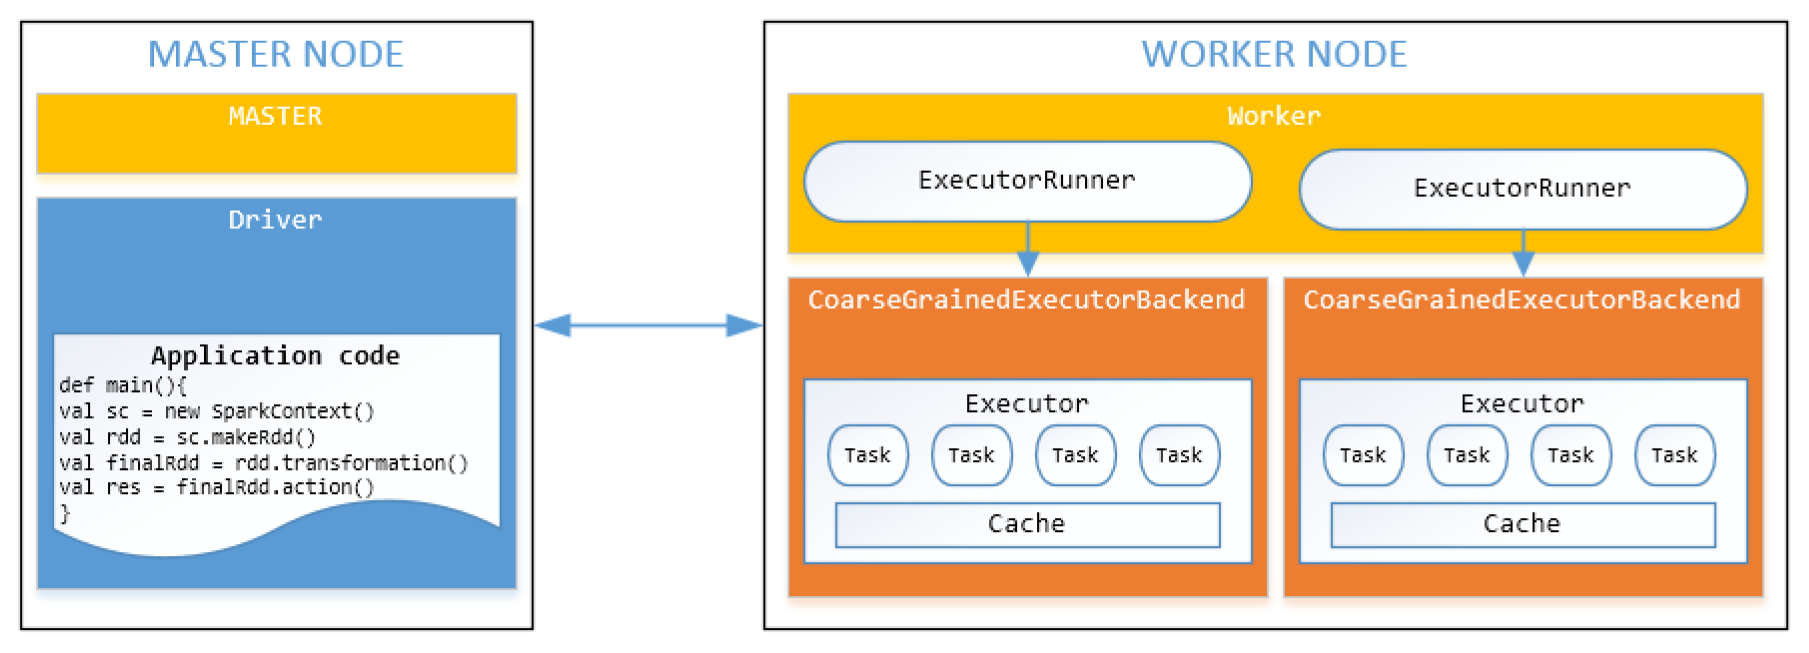
\includegraphics[width=\linewidth]{images/masterworker.png}
		\caption{\textit{Master node and Worker nodes.}}
	\end{figure}
	\begin{table}[H]
		\centering
		\begin{tabular}{p{0.47\linewidth}p{0.47\linewidth}}
			\textbf{Hadoop} & \textbf{Spark} \\ \hline
			One task per UNIX process (JVM), more if there is JVM reuse. & Tasks run in one or more threads within a single UNIX process (JVM). \\ \hline
			Use MultiThreadedMapper advanced feature to have threads in Map tasks. & Executor process is statically allocated to worker, even with no threads. \\ \hline
			\textbf{Short-life executor with one large task.} & \textbf{Long-life executor with many small tasks.} \\ \hline
		\end{tabular}
	\end{table}
	\subsection{Benefits of the Spark architecture}
		\subsubsection{Isolation}
			\par
			Applications are completely isolated, task scheduling per application.
		\subsubsection{Low-overhead}
			\par
			The task setup cost is that of spawning a thread, not a process. Small tasks mitigate the effects of data skew (difference in the distribution of data).
		\subsubsection{Sharing data}
			\par
			Applications cannot share data in memory natively, they use an external storage service like a distributed caching mechanism to store and share RDDs in memory.
		\subsubsection{Resource allocation}
			\par
			Static process provisioning for executors (even without active tasks) and dynamic provisioning under development.
			
\section{Resilient Distributed Datasets}
	\subsection{What is an RDD}
		\par
		RDDs are partitioned, locality aware, distributed collections. RDDs are immutable.
		\newline
		RDDs are data structures that either point to a direct data source (HDFS) or apply some transformations to its parent RDD(s) to generate new data elements.
		\newline
		Computations on RDDs are represented by lazy evaluated lineage DAG, composed by chained RDDs.
	\subsection{RDD abstraction and interfaces}
		\par
		The objective is to simplify scheduling, avoid to modify the scheduler for each operator. RDDs support a wide array of operators (more than just Map and Reduce) and allow arbitrary composition of them.
		\newline
		\par\noindent
		The RDD interfaces are:
		\newline
		\textbf{Set of partitions ("splits")}, like in Hadoop, each RDD is associated to (input) partitions.
		\newline
		\textbf{List of dependencies on parent RDDs}, completely new with respect to Hadoop.
		\newline
		\textbf{Function to compute a partition given the parents}, "user defined code".
		\newline
		\textbf{Optional preferred locations}, to enforce data locality.
		\newline
		\textbf{Optional partitioning info (Partitioner)}, in case you want to pay attention to the behaviour of the shuffle mechanism\footnote{This is done with second order functions, like \textit{groupby}.}.
	\pagebreak
	\subsection{RDD examples}
		\par\indent
		\par\textbf{Hadoop RDD}
		\begin{table}[H]
			\centering
			\begin{tabular}{p{0.3\linewidth}p{0.64\linewidth}}
				\textbf{partitions} & one per HDFS block \\
				\textbf{dependencies} & none, this is an input RDD \\
				\textbf{compute(partition)} & read corresponding block \\
				\textbf{preferred locations} & HDFS block location, to maintain data locality \\
				\textbf{partitioner} & none \\
			\end{tabular}
		\end{table}
		\par
		\textbf{Filtered RDD}
		\begin{table}[H]
			\centering
			\begin{tabular}{p{0.3\linewidth}p{0.64\linewidth}}
				\textbf{partitions} & same as parent RDD \\
				\textbf{dependencies} & one to one on parent \\
				\textbf{compute(partition)} & compute parent and filter it \\
				\textbf{preferred locations} & none, ask parent \\
				\textbf{partitioner} & none \\
			\end{tabular}
		\end{table}
		\par
		\textbf{Joined RDD}
		\begin{table}[H]
		\centering
		\begin{tabular}{p{0.3\linewidth}p{0.64\linewidth}}
			\textbf{partitions} & one per reduce task \\
			\textbf{dependencies} & shuffle on each parent, data can come from any machine \\
			\textbf{compute(partition)} & read and join shuffled data \\
			\textbf{preferred locations} & none, data can come from anywhere \\
			\textbf{partitioner} & HashPartitioner(numTask), spark knows this data is hashed \\
		\end{tabular}
		\end{table}
	\subsection{RDD dependecy types}
		\par
		We define a \textbf{narrow dependency} when each partition of the parent RDD is used by at most one partition of the child RDD. Narrow dependencies are exploited for optimization, tasks can be executed locally without shuffle (map, filter, union, join with co-partitioned inputs).
		\newline
		\par\noindent
		There is a \textbf{wide dependency} when multiple child partitions may depend on one partition of the parent RDD. This means we have to shuffle data unless the parents are hash-partitioned (sortbykey, reducebykey, groupbykey, join with non co-partitioned inputs).
		\newline
		\par\noindent
		The DAG scheduler optimizes Stages and Tasks before submitting them to the Task scheduler: \textbf{pipelining narrow dependencies within a stage, selecting the join plan based on partitioning, reusing cached data}.
	\subsection{Operations on RDDs: Transformations and Actions}
		\par
		Transformations are set of operations on an RDD that define how they should be transformed. As in relational algebra, the application of a transformation to an RDD yields a new RDD (because RDDs are immutable). Transformations are lazily evaluated to allow optimization to take place before execution. Caching is a transformation, transformations return type is an RDD.
		\newline
		\par\noindent
		Actions apply transformation chains on RDDs, eventually performing some additional operations. Some actions only store data to an external source (HDFS), others fetch data from the RDD (and its transformation chain) upon which the action is applied, and convey it to the driver\footnote{Take care when conveying information to the driver, it could be too much data and it could not fit in memory.}. Actions return type is a built-in scala/java type.
\section{Spark Word Count}
	\subsubsection*{The driver}
		\par
		A SparkContext initializes the application driver, the latter then registers the application to the cluster manager and gets a list of executors. Finally the driver takes full control of the Spark Job.
	\subsubsection{The code}
		\par 
		RDD lineage DAG is built on driver side with data source RDDs and transformation RDDs (creates by transformations). An action triggers the DAG scheduler to submit a job\footnote{The \textit{sortbykey} transformation is an exception, it issues a job too.}.
		\begin{figure}[h!]
			\centering
			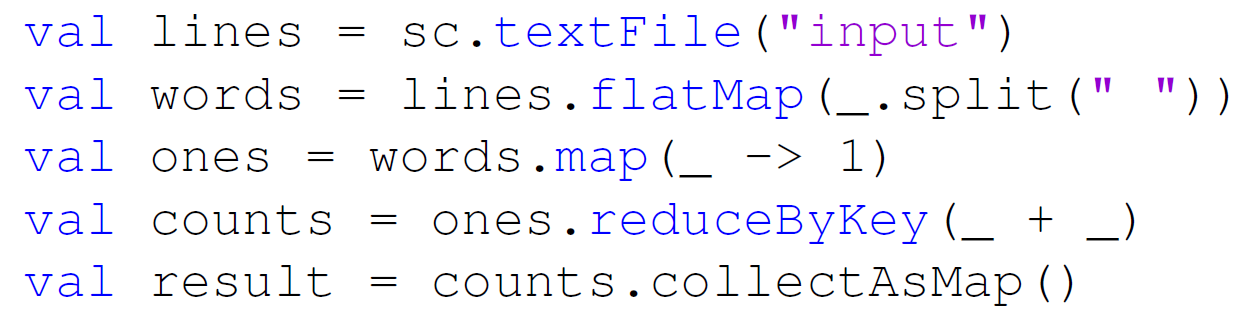
\includegraphics[width=\linewidth]{images/sparkwc.png}
			\caption{\textit{Spark word count code.}}
		\end{figure}
	\subsubsection{The DAG}
		\par
		The Directed Acyclic Graph is built from the RDD lineage. The DAG scheduler transforms the DAG into stages and turns each partition of a stage into a single task.
		\newline
		Spark tuning is the repartitioning of the initial data to fully exploit the hardware: make more tasks for more, smaller, partitions, instead of just one big partition on one task.
	\subsubsection{The execution plan}
		\par
		Spark Tasks execute serialized RDD lineage DAG plus the closures of transformations. They are run by Spark Executors.
		\newline
		The driver side task scheduler launches tasks on executors according to resources and locality constraints, it decides where to run tasks.
	\subsubsection{The Shuffle phase}
		\par
		The \textit{reducebykey} transformation induces the shuffle phase (wide dependency), intermediate key-value pairs are stored on the local file system like in Hadoop.
		\newline
		This transformation also implements map-side combiners to pre-aggregate data.
\chapter{Cluster Schedulers}

\section{Cluster Scheduling Principles}
	\subsubsection{Scheduling}
	Cluster \textbf{utilization }and \textbf{efficiency }are key indicators for good \textbf{resource management }and \textbf{scheduling decisions}. A better scheduling means smaller clusters as well as larger workloads with the same cluster size.
	\subsubsection{Multiplexing}
	The multiplexing of multiple, heterogeneous mixes of applications running concurrently complicates the scheduling problem.
	\subsubsection{Scalability}
	Cluster and workload size keep growing, and the scheduling complexity is roughly proportional to the cluster size. Schedulers must be scalable and bottlenecks have to be avoided.
	\subsubsection{Workload}
	The cluster scheduler must support heterogeneous workloads and clusters.\newline
	Clusters are made of several generations of machines and the workload evolves in time and is made of different applications. Generally there are two main job types: \textbf{batch jobs} (e.g. MapReduce computations) and \textbf{service jobs} (e.g. end-user facing a web service).\newline
	Knowing the workload of a cluster is fundamental, measurements can inform scheduling design, for example, about the differences between jobs in terms of number and runtime.

\section{Taxonomy of scheduling design issues}
	\textbf{Work Partitioning}\newline
	How to allocate work across frameworks: workload oblivious load balancing; partitioned workload and specialized schedulers; hybrid.\newline
	\newline
	\textbf{Resources choice}\newline
	Which clusters resources are made available to concurrent networks: all resources available; a subset is granted or offered\footnote{In this case the use of preemption primitives helps scheduling primitives but it can cause a waste of work.}.\newline
	\newline
	\textbf{Interference}\newline
	What to do when multiple frameworks attempt to use the same resources: make sure to avoid conflicts, partition resources across frameworks (\textbf{pessimistic concurrency control}) or, detect and undo conflicts if there are any (\textbf{optimistic concurrency control}).\newline
	\newline
	\textbf{Allocation granularity}\newline
	Task scheduling policies: atomic, all-or-nothing gang scheduling (e.g. Message Passing Interface programs); or incremental placement, hoarding (e.g. MapReduce).\newline
	\newline
	\textbf{Cluster-wide behaviour}\newline
	Requirements that need a global view like \textbf{fairness across frameworks} and \textbf{global notion of priority}.

\section{Schedulers Architectures}
	\subsubsection{Monolithic}
	Uses a \textbf{single centralized instance} that implements all the policies in a single code base. It applies the \textbf{same scheduling algorithm to all incoming jobs}.\newline
	A possible alternative is to add the support for multiple paths for different jobs, implementing different scheduling logic.\newline
	It is difficult to implement (add new scheduling policies) and to maintain (does not scale well to large clusters).
	\subsubsection{Statically partitioned}
	This is the standard approach: each framework has complete control over a set of resources (e.g. Hadoop 1.0), a single resource manager grants resources to independent \textit{framework schedulers}.\newline
	It can schedule between \textbf{multiple frameworks} but it has to deal with the problems of static partitioning: \textbf{fragmentation of resources} and \textbf{sub-optimal utilization} of the cluster.
	\begin{figure}[H]
		\centering
		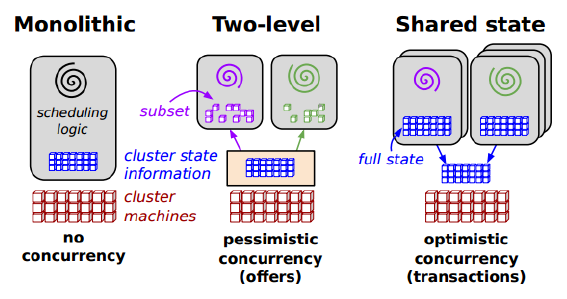
\includegraphics[width=0.5\linewidth]{images/clust_sched_arch.png}
		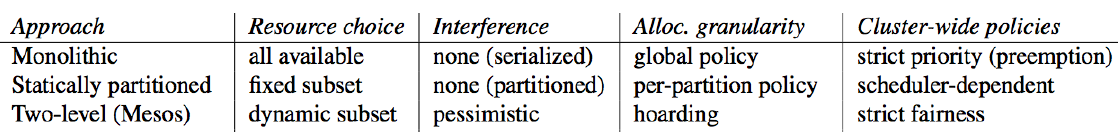
\includegraphics[width=\linewidth]{images/clust_sched_comparison.png}
		\caption{\textit{Comparison of cluster scheduling approaches.}}
	\end{figure}
	\subsubsection{Two-levels}
	It uses a \textbf{coordinator} to \textbf{dynamically allocate resources} to concurrent frameworks.\newline
	An example is \textbf{Mesos}, it makes exclusive resource offers to the frameworks, they lock resources by acccepting the offers (pessimistic concurrency control). No global cluster state is available to frameworks.\newline
	The \textbf{YARN} scheduler is closer to a monolithic architecture. It has a centralized resource allocator (RM) with per-job framework master (AM), but the latter only provides job management services (no scheduling).
	\subsubsection{Shared-state}
	Multiple replicas of cluster state are independently updated by application-level schedulers. After the change is applied locally, the scheduler issues an optimistically concurrent transaction to update the shared cluster state (e.g. Google's Omega).

\section{YARN}
	\subsection{Previous limitations and improvements}
		\subsubsection{Hadoop 0.1 limitations}
		It \textbf{only supports MapReduce} and it has \textbf{scalability issues}. System failures destroy running and queued jobs (\textbf{poor availability}). \textbf{Sub-optimal resource utilization}: static partitioning of resources in Map or Reduce slots.
		\subsubsection{YARN improvements}
		\textbf{Support for multiple applications}. Separate resource management from application logic and share same Hadoop cluster across applications.\newline
		\newline
		\textbf{Improved cluster utilization}. Generic resource \textit{container} model replaces fixed Map/Reduce slots. Container allocation based on locality and memory.\newline
		\newline
		\textbf{Improved scalability}. Remove complex application logic from the resource manager. Compact scheduling protocol. Message passing based on loosely coupled design.\newline
		\newline
		\textbf{Application agility}. Use protocol buffers for RPC (Remote Procedure Call) gives wire compatibility. MapReduce becomes an application in user space. Multiple versions of an application can co-exist. Easier upgrade of framework and applications.\newline
		\newline
		\textbf{Shared services}. Common services in a pluggable framework. Distributed file sharing service. Remote data read service. Log aggregation service.
		 
	\subsection{Architecture and Core Components}
	Nodes resources are allocated to applications on request (\textbf{dynamic resource partitioning}), there are no more slots.\newline
	Separate resource management from application logic: cluster-wide resource allocation and management with per-application master component.
		\subsubsection{Schedulers}
		Schedulers are pluggable components of the RM, in addition to the existing ones, advanced scheduling is supported. Currently supported schedulers are the capacity scheduler and the fair scheduler, it also supports Dominant Resource Fairness and Hierarchical Queues.
		\subsubsection{Resource Manager [RM]}
		The RM runs on the master node and arbitrates system resources between competing applications.\newline
		It tracks heartbeats from Node Managers (\textbf{Node management}).\newline
		It handles to the Application Master the requests for new containers and de-allocates them when they expire or the application finishes (\textbf{containers management}).\newline
		It creates a container for each new AM and tracks its health (\textbf{AM management}).\newline
		It integrate Kerberos (\textbf{Security management}).
		\subsubsection{Node Manager [NM]}
		The Node Manager runs on slave nodes, it \textbf{handles communications with the RM}: it registers, monitors and communicates node resources, and sends heartbeats and container status.\newline
		It \textbf{manages processes in containers}: launches AMs on request from the RM and launches applications on request from the AMs. Furthermore, it \textbf{monitors resource usage and kills processes and containers}.\newline
		Finally, it p\textbf{rovides log services}: Log Aggregation and roll over to HDFS.\newline
		The shuffle mechanism is an auxiliary service that runs un the NM JVM as a persistent service.
		\subsubsection{Resource containers}
		They are created by the RM upon request. They allocate a certain amount of resources on slave nodes for the applications to run.\newline
		The container launch context contains a container ID, the commands to start the application task, the environment configuration and local resources (application binary, HDFS files).
		\subsubsection{Application master [AM]}
		It is application specific, it runs in a container and requests one or more containers to execute application tasks.\newline
		A \textbf{resource request} contains a resource name (hostname, rackname, *), a priority (within the same application), resource requirements (memory, CPU) and the number of containers needed.
	\subsection{Fault tolerance}
		\subsubsection{Container failure}
		The AM reattempts containers that complete with exceptions or fails. Applications with too many failed containers are considered failed.
		\subsubsection{AM failure}
		If the application or the AM fails, the RM will re-attempt the whole application. Optionally the \textit{job recovery} could be set, it uses state to find which containers succeeded and which failed, and reschedules only the latter.
		\subsubsection{NM failure}
		If NM stops sending heartbeats; the RM removes it from the active nodes list and reschedules the containers on the filed node. AMs on the failed node are resubmitted completely.
		\subsubsection{RM failure}
		No application can be run if the RM is down. It can work in active/passive mode (like the Name Node of HDFS).
	
\section{MESOS}
	\subsection{Introduction and Motivations}
	Clusters of commodity servers are a major
	computing platform. To simplify the programming of the cluster, a diverse array of	cluster computing frameworks have been developed, but no framework will be optimal for all applications. Therefore, it is necessary to run multiple frameworks in the same cluster.\newline Multiplexing a cluster between frameworks improves utilization and	allows applications to share access to large datasets that	may be too costly to replicate across clusters. Two solutions for sharing a cluster are either to statically partition the cluster or to allocate a set of VMs to each
	framework. Unfortunately, these solutions achieve neither
	high utilization nor efficient data sharing. The main
	problem is the mismatch between the allocation granularities
	of these solutions and of existing frameworks.\newline
	\newline
	The short duration of tasks and the ability to run multiple tasks per node allow jobs to achieve high data locality, as each job will quickly get a chance to run on nodes storing its input data. Short	tasks also allow frameworks to achieve high utilization,	as jobs can rapidly scale when new nodes become available.
	Unfortunately, because these frameworks are developed
	independently, there is no way to perform fine grained
	sharing across frameworks, making it difficult to
	share clusters and data efficiently between them.\newline
	\newline
	A centralized approach would need to take as input framework requirements, resource availability, and organizational policies,
	and compute a global schedule for all tasks. This approach has to face several challenges.\newline
	The scheduler would need to provide a sufficiently expressive
	API to capture all frameworks’ requirements, and
	to solve an online optimization problem for millions
	of tasks. Even if such a scheduler were feasible, this
	complexity would have a negative impact on its scalability
	and resilience. Moreover, many existing
	frameworks implement their own sophisticated scheduling, and moving this functionality to a global
	scheduler would require expensive refactoring.\newline
	\newline
	Mesos uses a decentralized approach: it delegates
	control over scheduling to the frameworks. This is accomplished through the abstraction of \textit{resource
	offer}.\newline
	Mesos decides how many resources to offer each framework,
	while frameworks decide which resources to accept
	and which tasks to run on them. This decentralized
	scheduling model allows frameworks to meet
	goals such as data locality nearly perfectly. In addition,
	resource offers are simple and efficient to implement, allowing Mesos to be highly scalable and robust to failures.\newline
	\newline
	The typical workloads in data warehouse systems using Mesos includes: heterogeneous MapReduce jobs, production and had-hoc queries; large scale machine learning; SQL-like queries.
	\subsection{Architecture}
	The design philosophy is to have a scalable and resilient core exposing low level interfaces and to use high level libraries for common functionalities.\newline
	Mesos manages cluster resources while the frameworks control task scheduling and execution.\newline
	The two levels approach lets frameworks be independent so that they can support diverse scheduling requirements.
		\subsubsection{Mesos Master}
		It implements the first level scheduling. It uses resource offers (lists of free resources on multiple slaves) to implement fine-grained sharing. It collects resource utilization from slaves and implements cluster-wide allocation policy (Fair Sharing or Priority based).\newline
		Mesos also implements filters to optimize the resource offers mechanism (filter based on machine or resources). Frameworks can decide to reject an offer and wait for offers satisfying application constraints.\newline
		The master incentives the frameworks to speed up the offers mechanism by counting offers to a framework, it can also decide to invalidate an offer to avoid blocking or misbehaviours.
		\subsubsection{Mesos Frameworks}
		Each framework decides how to execute a job and its tasks\footnote{The actual task execution is requested by the master.}. Each framework has one scheduler and one executor per application. The framework scheduler registers to the master, selects which offer to accept and describes the tasks to launch on accepted resources.\newline
		The framework executor is launched on Mesos slaves executing on accepted resources, it takes care of running the framework's tasks.
		\subsubsection{Resource allocation and revocation}
		Resource allocation is done through a pluggable allocation module which can use either max-min fairness or strict priority.\newline
		It works under the assumption that tasks are short because Mesos only reallocates resource when tasks finish.\newline
		Unfortunately some jobs (e.g. streaming) may have long tasks, in this case Mesos can kill running tasks. Some applications (e.g. MPI) may be harmed by this mechanism more than others (e.g. MapReduce), therefore Mesos implements a guaranteed allocation mechanism: a minimum set of resources granted to a framework, if a framework is below his guaranteed allocation then Mesos never kills tasks, otherwise it could kill any of them.
		\subsubsection{Performance Isolation}
		Isolation between executors on the same slave is achieved through low-level OS primitives (pluggable isolation module). The currently supported mechanisms can limit CPU, memory, network and I/O bandwidth using Linux Containers and Solaris Cages.\newline
		This approach offers better isolation than the previous process-based approach but fine grained isolation is not yet fully functional.
		\subsubsection{Fault Tolerance}
		The master is designed with a soft state containing the list of active slaves, the list of registered frameworks and the list of running tasks.\newline
		Multiple masters stay in a hot-standby mode handled by zookeeper, upon failure a new master is elected (\textit{leader election}), slaves and executors help populate the new master's state.\newline
		In order to help frameworks tolerate failures, the master send health reports to the schedulers and allows multiple schedulers for a single framework.
	\subsection{Behaviour}
	The ideal Mesos workload has elastic frameworks, supporting scaling up and down seamlessly. Tasks duration has to me homogeneous and short and there has to be no strict preference over cluster nodes.\newline
	In the case a framework has cluster node preferences, Mesos can emulate a centralized scheduler offering cluster and framework wide resource sharing.
		\subsubsection{Definitions and metrics}
		\textbf{Elasticity} describes the capacity of a workload to use resources as soon as they are acquired and release them as soon as tasks finish.\newline
		\textbf{Task runtime distribution} measures homogeneity/heterogeneity of a workload.\newline
		\textbf{Mandatory resource} are required by a framework to work (assumption: mandatory resources < guaranteed share).\newline
		\textbf{Preferred resources} are resources that a framework should acquire to achieve better performance but are not fundamental for the job to work.\newline
		\newline
		\textbf{Framework ramp-up time} is the time it takes a new framework to get its fair share.\newline
		\textbf{Job completion time} is the time it takes a job to complete (assuming one job per framework).\newline
		\textbf{System utilization} is the total cluster resources utilization, with focus on CPU and memory.
		\subsubsection{Homogeneous and heterogeneous tasks}
		When dealing with a homogeneous workload there exist two cases: if there is a configuration satisfying all frameworks constraints the system will eventually converge to this optimal allocation; if no such allocation exists (e.g. demand is larger than supply) then lottery scheduling is used to achieve a weighted fair allocation.\newline
		If Mesos is dealing with an heterogeneous workload, then the worst case scenario happens when all nodes required by a short job are filled with long tasks. Fortunately the probability of such an event is small.
		\subsubsection{Limitations of Distributed Scheduling}
		\textbf{Fragmentation}: distributed collection of frameworks might not achieve the same packing quality of a centralized scheduler, this is mitigated by the use of big nodes (many CPUs, many cores) running small tasks.\newline
		\textbf{Starvation}: Large jobs may wait indefinitely for slots to become free because they are monopolized by small tasks from small jobs. This is mitigated by a \textit{minimum offer size} mechanism.
		
\section{BORG}
	\subsection{Introduction}
	Borg provides three main benefits: it \textbf{hides the details
	of resource management and failure handling} so its users can
	focus on application development instead; \textbf{operates with very high reliability and availability}, and supports applications that do the same; and lets us \textbf{run workloads across
	tens of thousands of machines effectively}.
	
	\subsection{User Perspective}
	Users submit their work to Borg	in the form of \textit{jobs}, each of which consists of one or more
	\textit{tasks} that all run the same program (binary). Each job runs in one Borg \textit{cell}, a set of machines that are managed as a
	unit.
		\subsubsection{Workloads}
		Borg cells run a heterogenous workload with two main parts.\newline
		The first is \textbf{long-running services} (mostly production, high-priority) that should “never” go down, and handle short-lived latency-sensitive requests (end-user-facing products such as Gmail or Google Docs).\newline
		The second is \textbf{batch jobs} that take from a few seconds to a few days to complete; these are much less sensitive to short-term performance fluctuations.\newline
		\newline
		The workload mix varies across cells, which run different mixes of applications depending on their major tenants (e.g., some cells are quite batch-intensive), and also varies over time: batch jobs come and go, and many end-user-facing service jobs see a	diurnal usage pattern. 
		\subsubsection{Clusters and cells}
		The machines in a cell belong to a single cluster, defined by the high-performance datacenter-scale network fabric that connects them.\newline
		A cluster lives inside a single datacenter building, and a collection of buildings makes up a site. A cluster usually hosts one large cell and may have a few	smaller-scale test or special-purpose cells (to avoid any single point of failure).\newline
		\newline
		The machines in a cell are heterogeneous. Borg isolates	users from most of these differences by determining	where in a cell to run tasks, allocating their resources, installing their programs and other dependencies, monitoring	their health, and restarting them if they fail.
		\subsubsection{Jobs and tasks}
		A Borg job’s properties include its \textbf{name}, \textbf{owner}, and the \textbf{number of tasks} it has. Jobs can have \textbf{constraints} (hard or soft) to force its tasks to run on machines with particular attributes.\newline
		\newline
		Each task maps to a set of Linux processes running in a container on a machine in a Borg cell.\newline
		\newline
		A task has properties too, such as its \textbf{resource requirements} and the \textbf{task’s index} within the job. Most task properties are the same across all tasks in a job, but can be overridden.\newline
		Tasks can \textbf{run on any resource dimension}: there are no fixed-size buckets or
		slots.\newline
		\newline
		Borg implements a declarative configuration language (BCL) to specify jobs and tasks. It uses lambda functions to allow calcuations, application description can be over 1k loc.\newline
		\newline
		\begin{figure}[H]
			\centering
			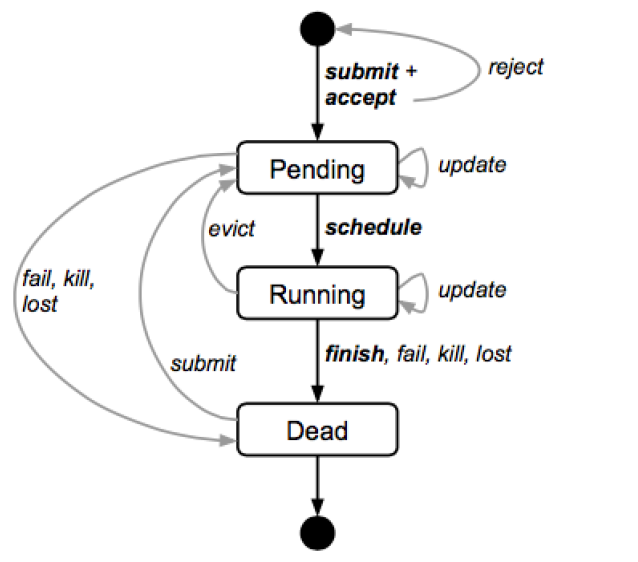
\includegraphics[width=0.5\linewidth]{images/borg_job_state_diagram.png}
			\caption{\textit{State diagram for both jobs and tasks. Users can trigger submit, kill, and update transitions.}}
		\end{figure}
		Users can interact with live jobs, this is achieved mainly using RPC. They can \textbf{update the specification of tasks}, while their parent job is running, updates are non-atomic and executed in a rolling-fashion.\newline
		Some task updates (e.g., pushing a new binary) will always require the task to be restarted; some (e.g., increasing resource requirements or changing constraints) might make the task no longer fit on the machine, and cause it to be stopped and rescheduled; and some (e.g., changing priority) can always be done without restarting or moving the task.
		\subsubsection{Allocs}
		A Borg alloc (short for allocation) is a \textbf{reserved set of resources on a machine} in which one or more tasks can be run; \textbf{the resources remain assigned whether or not they are
		used}.\newline
		Allocs can be used to set resources aside for future	tasks, to retain resources between stopping a task and starting it again, and to gather tasks from different jobs onto the	same machine.\newline
		An alloc \textit{set} is like a job: it is a group of allocs that reserve resources on multiple machines. \textbf{Once an alloc set has been created, one or more jobs can be submitted to run in it}.
		\subsubsection{Priority, Quota and Admission control}
		These are mechanisms to deal with resource demand and offer when more work shows up than can be accommodated (this is not scheduling, it is more admission control).\newline
		Job priorities are divided in non-overlapping bands for different uses, tasks from high-priority jobs can preempt low-priority tasks. Cascade preemption is avoided by disabling it for same-band jobs.\newline
		\newline
		Job/User quotas are used to decide which job to admit for scheduling. They are expressed as a vector of resource quantities at a given priority, for a period of time.\newline
		Pricing is the underlying mechanism to regulate user behaviour, it aligns user incentives to better resource utilization and discourages over-buying by over-selling quotas at lower priority.
		\subsubsection{Naming services}
		The Borg Name Service (BNS) is a mechanism to assign a name to tasks starting from cell name, job name and task number.\newline
		It uses the Chubby coordination service, it writes task names, health information and status. It is used by Borg RPC mechanism to establish communication	endpoints.\newline
		The DNS service inherits from BNS.
		\subsubsection{Monitoring services}
		Almost every task in Borg has a built-in HTTP server that provides health information and performance metrics.\newline
		The SIGMA service provides a monitoring UI with state of jobs, cells and tasks.\newline
		If a job is not running	Borg provides a “why pending?” annotation, together with guidance on how to modify the job’s resource requests to better fit the cell ("debugging service").\newline
		Billing services use monitoring information to compute usage-based charging, they help users debug their jobs and are used for capacity planning.
	\subsection{Architecture}
		\subsubsection{Borg master}
		The Borgmaster is one per Borg Cell, it orchestrates cell resources. It is composed of the \textbf{Borgmaster process} and the \textbf{scheduler process}.\newline
		The Borgmaster process handles client RPCs that either mutate state or lookup for state. It manages the state machines for all Borg “objects” (machines, tasks, allocs...), communicates with all Borglets in the cell and provides a Web-based UI.\newline
		\newline
		Borgmaster \textbf{reliability is achieved through replication}: the single logical process is replicated 5 times in a cell. The \textbf{master is elected using Paxos} when starting a cell, or upon failure of the current master. The Master serves as Paxos leader and cell state mutator.\newline
		Borgmaster replicas maintain an \textbf{in-memory} fresh copy of the cell state, they persist their state to a distributed Paxos-based store and help building the most up-to-date cell state when a new master is elected.\newline
		\newline
		Borgmaster \textbf{checkpoints its state} (time-based and event-based mechanism). The state includes everything related to a cell.\newline
		Checkpoints are used to restore the state to a functional one, e.g. before a failure or a bug, study a faulty state and fix it by hand, build a persistent log of events for future queries or for offline simulations.\newline
		\newline
		The \textbf{fauxmaster} is a high-fidelity simulator, it reads checkpoint files, accepts RPCs to make state machine changes and connects to simulated Borglets that replay real interactions from checkpoint files.\newline
		It helps users debug their application, make capacity planning, e.g. “How many new jobs of this type would fit in the cell?” and perform sanity checks for cell configurations, e.g. “Will this new configuration evict any important jobs?”.
		\subsubsection{Scheduling}
		New submitted jobs are stored in the Paxos store (for reliability) and put in the \textit{pending queue}. The scheduler process \textbf{operates at the task level}, it scans asynchronously the pending queue and assigns tasks to machines satisfying constraints.\newline
		The scanning is based on priority, within the same class, scheduling uses a round robin mechanism to ensure fairness and avoid blocking.\newline
		\newline
		The scheduling algorithm has two main processes. The \textbf{feasibility checking} finds a set of machines that meet the task's constraints (including resources already assigned to lower priority tasks).\newline
		The \textbf{scoring} process ranks machines from the previous one in order to minimize the number and priority of preempted tasks, prefer machines with a local copy of task's binaries and dependencies, spread tasks across failure and power domains, and mix high and low priority tasks on the same machine (to allow the former ones to expand).\newline
		\newline
		The scoring mechanism used to work with \textbf{worst-fit scoring}: it minimized the change in cost when placing a new task, this approach its good to spread tasks, it leaves headroom for load spikes but leads to fragmentation.\newline
		A better approach is the \textbf{best-fit scoring} which leaves empty machines that can be used for large tasks but, on the other hand, makes it difficult to deal with load spikes as the headroom in each machine highly depends on load estimation.\newline
		The solution used in practice is an hybrid which tries to reduce the amount of stranded resources.\newline
		\newline
		One of the most important metrics to optimize is the \textbf{startup latency} (time from job submission to running task), it deeply \textbf{depends on binaries and package installation}, therefore a possible solution is to place tasks on machines that already have dependencies installed.
		\subsubsection{Borglet}
		The Borglet is a Borg agent present on every machine in a cell.\newline
		It starts and stops tasks, and restarts failed tasks.\newline
		It manages machine resources interacting with the OS.\newline
		It maintains and rolls over debug logs.\newline
		It reports the state of the machine to the Borg master.\newline
		\newline
		Interaction with the Borg master uses a pull-based mechanism (heartbeat like), the Borglet continues operating even if the communications are interrupted. A failed Borgled is blacklisted and all its tasks are rescheduled.\newline
		The Borg master as to perform \textbf{flow and rate control} to avoid message flooding and many borgmaster replicas receive state updates. In order to handle the message overhead, the \textbf{link shard mechanism} is used: each replica communicates with a subset of the cell (partitioning is computed at each leader election), and the link shard mechanism aggregate state information. Differential state update is used to reduce the load of the master.
		\subsubsection{Scalability}
		Scalability is achieved through the decentralized design: the scheduler process is separated from the Borg master process and there is one scheduler per Borg master replica. Scheduling is somehow decentralized and states changes are communicated from replicas to the elected Borg master that finalized the state update.\newline
		Additional techniques are used to improve scalability: score caching, equivalence class and relaxed randomization.
	\subsection{Behaviour}
		\subsubsection{Availability}
		In large scale systems, failure are the norm. The baseline techniques to achieve high availability are replication, checkpointing and storing persistent state in a distributed file system.\newline
		Some additional techniques are: automatic rescheduling of failed tasks, mitigating correlated failures, rate limitation, avoid duplicate computation, admission control to avoid overload and minimization of external dependencies for task binaries.
		\subsubsection{System Utilization}
		To measure system utilization a sophisticated metric is used: \textbf{Cell Compaction}. The fauxmaster is used to compute it: given a workload in a point in time, remove physical machines at each iteration and exit the loop when the workload can no longer fill the cell size.\newline
		\newline
		\textbf{Cell sharing} has its benefits: Borg can reclaim resources unused by production jobs.\newline
		\textbf{Large cells} can accommodate large jobs and avoid fragmentation too.\newline
		Borg users specify job's requirement in terms of \textbf{fine-grained resource requests}, fixed size containers would require more machines in a cell.\newline
		Borg uses a \textbf{resource reclamation} system and it builds estimates of resource usage called \textbf{resource reservations}. Production jobs only rely on resources limits.
		\subsubsection{Isolation}
		Many tasks may interfere with each other, to obtain performance isolation borglets operate on the OS to control Linux containers resources, assigning resources based on predicted future usage or memory pressure.\newline
		Additional techniques are: application classes (latency sensitive or batch), resource classes (compressible or non-compressible) and OS tuning, especially the OS scheduler.
	\subsection{Lesson Learned}
		\subsubsection{The bad}
		The job abstraction is to simplistic, multi-job services cannot be easily managed or addressed.\newline
		The addressing service is critical, one IP address implies managing ports as a resource, which complicates tasks.\newline
		Borg is more geared to power users than casual ones.
		\subsubsection{The good}
		Allocs are a useful resource envelope for one or more containers sharing resources and co-scheduled on the same machine.\newline
		Cluster management is more than task management.\newline
		Introspection is vital for debugging, capacity planning and monitoring.\newline
		The cooperation of micro-services that use a common low-level API to process requests and manipulate state is good.
	
\chapter{SparkSQL}

\section{Relational Algebra}	
	\subsection{Operators}
		\par
		Relational algebra operators are a operations on data that fit well the relational algebra model.
		\newline
		In traditional RDBMS, queries involve retrieval of small amounts of data while now we should keep in mind the workload underlying MapReduce: full scans of large amounts of data and queries that process all data (not selective\footnote{This is true in general. Most ETL jobs (Extract Transform Load) involve selection and projection to do data preparation.}).
		\newline
		Relations\footnote{A relation is a table.} (however big) can be stored in a distributed file system, if they don't fit in a single machine, they're broken into pieces.
		\subsubsection{Selection $\sigma_C(R)$}
			\par
			Apply a condition \textit{C} to each tuple of relation \textit{R}.
			\newline
			Produce in output a relation containing only tuples for the attributes\footnote{Attributes are the column headers of the table.} in \textit{S}.
		\subsubsection{Projection $\pi_S(R)$}
			\par
			Given a subset \textit{S} of attributes of a relation R, produce in output a relation containing only tuples for the attributes in \textit{S}.
		\subsubsection{Union, Intersection and Difference}
			\par
			Well known operators on sets, applied to the sets of tuples in two relations that have the same schema\footnote{The set of attributes $A_1, A_2, ..., A_n$ of a relation $R(A_1, A_2, ..., A_n)$ is called a schema.}.
		\subsubsection{Natural Join $R \bowtie S$}
			\par
			Given two relations, compare each pair of tuples, one for each relation. If the tuples agree on all the attributes common to both schema, then produce an output tuple that has components on each attribute, otherwise produce nothing.
			\newline
			The join condition can be on a subset of attributes.
		\subsubsection{Grouping and Aggregation $\gamma_X(R)$}
			\par
			Given a relation \textit{R}, partition its tuples according to their values in one set of attributes \textit{G} (grouping attributes). For each group, aggregate the values according to aggregation functions (SUM, COUNT, AVG, MIN, MAX) over other attributes.
			\newline
			\textit{X} is a list of elements that can be a grouping attribute or an expression $\theta(A)$, where $\theta$ is an aggregation function and \textit{A} is an attribute NOT among the grouping attributes.
			\newline
			The result is a relation with a tuple for each group. That tuple has a component for each of the grouping attributes with the common value of the tuples in that group, and another component for each aggregation function, with the aggregate value for that group\footnote{The COUNT function does not consider the values of an attribute, it just count the number of tuples. In SQL there is a COUNT DISTINCT operator to count the number of different values.}.
			
	\subsection{Operators and MapReduce}
		\subsubsection{Selection}
			\par
			Selection can be implemented in the map phase alone (but also in the reduce portion).
			\newline
			During the map phase, for each tuple \textit{t} in \textit{R}, check if \textit{t} satisfies the condition \textit{C}, if so, emit a key/value pair \textit{(t, t)}\footnote{There is no use for the second \textit{t}, it could be a 1 for a better implementation.}.
			\newline
			Then, use an identity reducer. We can't choose the number of mappers but we can choose the number of reducers, it is a matter of degree of parallelism. We can use a single reducer because it is a simple task, but if the reducer is loose (it makes a lot of pairs pass) then all of the pairs are going to hit just one machine so it is better to have multiple reducers.
			\newline
			The output is not exactly a relation because it does not have the same schema as the input.
		\subsubsection{Projection}
			\par
			In the map phase, for each tuple \textit{t} in \textit{R}, construct a tuple \textit{t'} by eliminating those components whose attributes are not in \textit{S}. Emit a key-value pair \textit{(t', t')}.
			\newline
			The reduce operation is duplicate elimination. For each key \textit{t'} produced by any of the map tasks, fetch \textit{t', [t', ..., t']} and emit a key-value pair \textit{(t', t')}.
			\newline
			The reducer operation is associative and commutative, so it is possible to optimize MapReduce by using a combiner in each mapper.
		\subsubsection{Union}
			\par
			Suppose the relations \textit{R} and \textit{S} have the same schema, the mappers don't do much, for each tuple \textit{t} in \textit{R} or \textit{S}, they emit a key-value pair \textit{(t, t)}.
			\newline
			Reducers do duplicate elimination, for each key \textit{t} there will be either one or two values, they emit \textit{(t, t)} in either case.
		\subsubsection{Intersection}
			\par
			Suppose the relations \textit{R} ans \textit{S} have the same schema, the map function is the same as for union, an identity mapper. During the reduce phase, if the key \textit{t} as value list \textit{[t, t]} (the key has been found two times), then emit the key-value pair \textit{(t, t)}, otherwise, emit \textit{(t, NULL)}.
		\subsubsection{Difference}
			\par
			Assume the relations \textit{R} and \textit{S} have the same schema, the only way a tuple \textit{t} can appear in the putput is if it is in \textit{R} but not in \textit{S}. The map function passes tuples from \textit{R} and \textit{S} to the reducer but it must also pass information about where the tuple came from.
			\newline
			In the map phase, emit tuples \textit{(t, 'R')} or \textit{(t, 'S')}.
			\newline
			In the reduce phase, for each key \textit{t}, if it is associated to \textit{'R'}, emit \textit{(t, t)}. Otherwise (it is associated to \textit{['R', 'S'], ['S', 'R'] or 'S'}), emit the key-value pair \textit{(t, NULL)}.
		\subsubsection{Join}
			\par
			Suppose we have two relations \textit{R(A, B)} and \textit{S(B, C)}, we must find tuples that agree on their \textit{B} components. We shall use the \textit{B-value} as the key, the value will be the other component and the name of the relation, so that the reducer knows from which relation each tuple is coming from.
			\newline
			In the map phase, for each tuple \textit{(a, b)} or \textit{(b, c)} emit the key-value pair \textit{(b, ('R', a))} or \textit{(b, ('S', c))}.
			\newline
			In the reduce phase, each key \textit{b} will be associated to a list of pairs that are either \textit{('R', a)} or \textit{('S', c)}. Emit pairs of the form $(b, [(a_1, b, c_1), (a_2, b, c_2), ..., (a_n, b, c_n)])$.
			\newline
			In general, for \textit{n} tuples in relation \textit{R} and \textit{m} tuples in relation \textit{S}, all with a common \textit{B-value}, we end up with \textit{nm} tuples in the result. Therefore if all tuples of both relations have the same \textit{B-value}, then we're computing the Cartesian product.
		\subsubsection{Grouping and Aggregation}
			\par
			Let \textit{R(A, B, C)} be a relation to which we apply $\gamma_{A, \theta(B)}(R)$, under the simplifying assumption of using one grouping attribute and one aggregation function, we know that: the map operation prepares the grouping, that is done by the framework, and the reducers compute the aggregation.
			\newline
			In the map phase, for each tuple \textit{(a, b, c)} emit the key/value pair \textit{(a, b)}.
			\newline
			In the reduce phase, each key represents a group, apply $\theta$ to the list $[b_1, b_2, ..., b_n]$ and emit the key-value pair \textit{(a, x)} where $x = \theta([b_1, b_1, ..., b_n])$.
	
\section{DataSource and DataFrame API}
	\par
	The DataSource API is used to \textbf{read and write from a variety of formats, either built-in or external}.
	\newline
	It has a unified interface: the functions read, load, write and save create new \textbf{I/O builders}. The builder methods are used to specify the data format, define data partitioning, handle existing data and more.
	\newline
	\par
	The idea of Dataframe is borrowed from Python Pandas: \textbf{tabular data with an API}. They are an abstraction for selecting, filtering, aggregating and plotting structured data.
	\newline
	The schema is applied only on read, not on write as traditional DBMS. Schema inference can be automatic, it is a distributed collection of rows organized into named columns.
	\newline
	The Dataframe \textbf{introduces structure to the data of the low-level RDD} and it specifies relational operators (select, join, aggregate, filter).
	\begin{figure}[H]
		\centering
		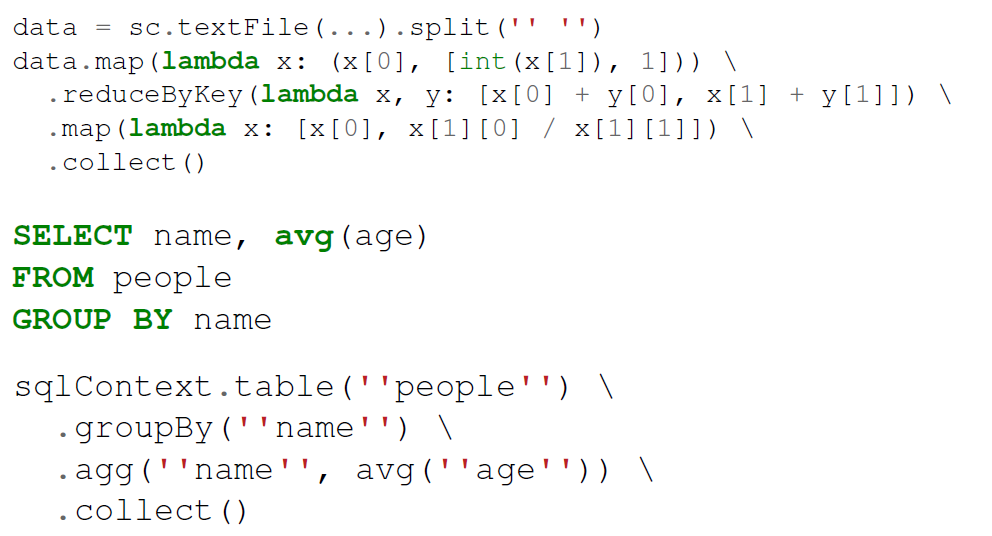
\includegraphics[width=0.8\linewidth]{images/dataframe.png}
		\caption{\textit{Comparison between RDDs, SQL and Dataframes.}}
	\end{figure}

\section{SparkSQL Architecture}
	SparkSQL borrows many ideas from traditional RDBMSs, it does optimization for efficiency and performance (logical plan and physical plan) using a sophisticated cost model (cost based or rule based).
	\begin{figure}[H]
		\centering
		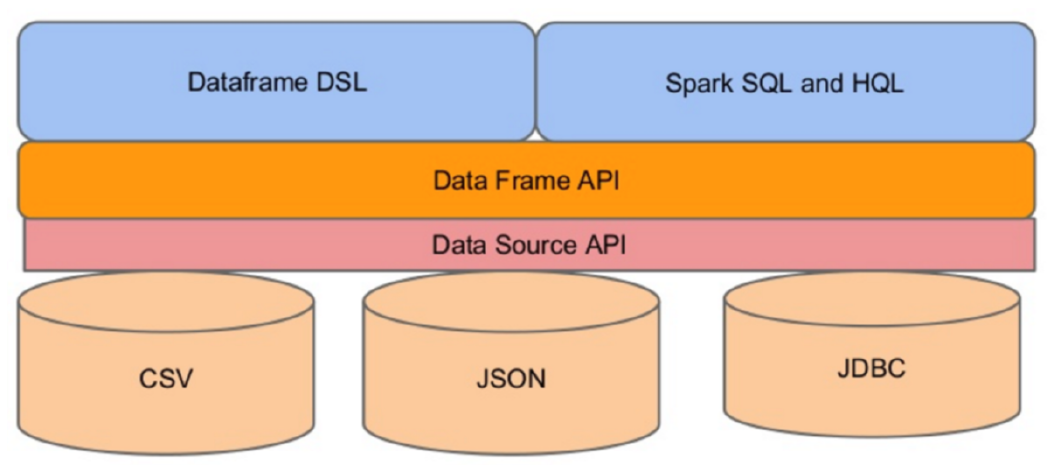
\includegraphics[width=0.8\linewidth]{images/sparksqlarch.png}
		\caption{\textit{Global view of SparkSQL architecture.}}
	\end{figure}
	The SparkSQLContext goes through a series of steps to get the data.\newline
	First, it builds an unresolved logical plan using the DataFrame and the SQL Abstract Syntax Tree. The AST then take information from a Catalog (e.g the name of attributes to reference the data) to produce a more human readable plan.\newline
	The logical plan (or tree) is optimized moving operators around, it defines the \textbf{logical flow of data from the extraction to the end}.\newline
	\begin{figure}[H]
		\centering
		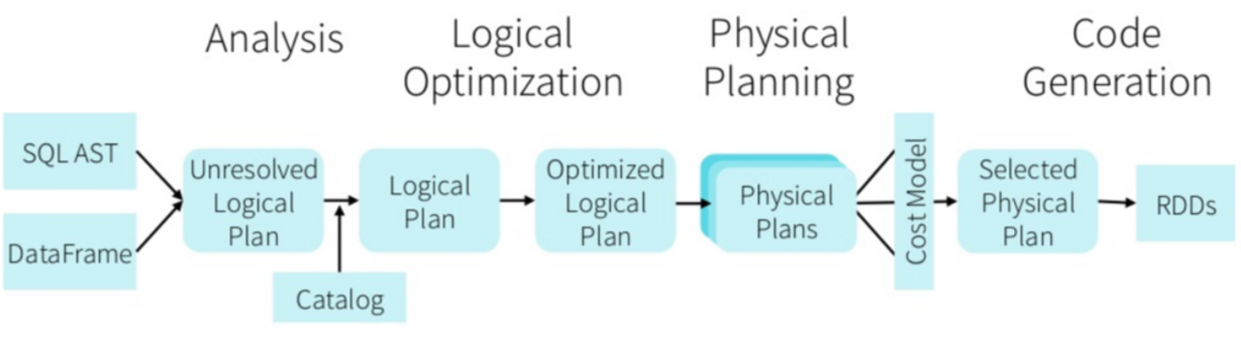
\includegraphics[width=0.8\linewidth]{images/sparksqlcontext.png}
		\caption{\textit{Flow of data through the SparkSQLContext.}}
	\end{figure}
	From the optimized logical plan a list is made of all the possible physical plans, these are then evaluated by a cost model which is continuously refined: it associates a cost to the operators and the cardinality.\newline
	Finally the selected physical plan is translated in Java ByteCode that will be submitted to the cluster.\newline
	\newline
	The \textbf{Catalyst optimizer} is the component taking care of these steps. It exploits some scala language features like \textit{Quasiquotes} for better tree manipulation.\newline
	\newline
	The \textit{project Tungsten} is a valid alternative that better exploits modern compilers, CPUs and cache locality. The more important feature is manages memory explicitly and eliminates the overhead of JVM object model and garbage collection.
	

\chapter{Distributed Storage Systems}

\section{The CAP Theorem}
	The CAP theorem relates the following three properties:
	\begin{itemize}
		\item \textbf{Consistency}: Every operation must appear to take effect in a single indivisible point in time between its invocation and response.
		\item \textbf{Availability}: Every client's request is served (receives a response) unless a client fails (despite a strict subset of server nodes failing).
		\item \textbf{Partition tolerance}: A system functions properly even if the network is allowed to lose arbitrarily many messages sent from one node to another.
	\end{itemize}
	To sacrifice P implies that the system does not function properly, therefore it sacrifices C or A. In the same way, negating P means that the system is not allowed to lose arbitrarily many messages, but in practice it is not possible to choose whether the network will lose messages or not.\newline
	In practical distributed systems partitions may occur and this is not under the system designer control. The designer choice is between C and A when/if temporary partitions occur.\newline
	In summary, \textbf{practical distributed systems are either CP or AP, the choice depends on the application logic}.

\section{Amazon Dynamo}
	\subsection{Overview}
	Amazon Dynamo is behind the Amazon Web Services. AWS is AP (sacrifices consistency), and follows the BASE philosophy (no ACID): Basically Available, Soft state, \textbf{Eventually consistent}.\newline
	Clearly, consistency violations have significant financial consequences and impact customer trust, but not in several Amazon services (billing is separated).\newline
	\newline
	Dynamo is an highly available key-value storage system that favours availability over consistency under failures.\newline
	It has a simple API (\textit{get(), put()}) that uses and additional argument to pass a \textit{context}, holding critical metadata (typically small).\newline
	Amazon Dynamo main features are:
	\begin{itemize}
		\item Low latency
		\item Scalability
		\item Always-on, available
		\item Partition and fault tolerance
		\item \textbf{Eventually} consistency
	\end{itemize}
	The design is made to have an \textbf{always writable} data store that allows multiple versions of data and \textbf{reconciles and resolves conflicts during reads}. Conflicts are solved depending on the business logic on the application size and in a deterministic way (last write) on the Dynamo side.\newline
	Failure detection is unreliable, the detection is triggered by read/write requests (in band detection), there is no dedicated component. \textbf{It does not make the distinction between faults and partitions}.
	\subsection{Data partitioning and consistent hashing}
	Dynamo uses dynamic partitioning of keys over a set of storage nodes (technique used for DHTs).\newline
	The hashes of keys give m-bit key identifiers and the hashes of nodes give m-bit node identifiers. Identifiers are ordered in a circle.\newline
	A key \textit{k} is assigned to the closest \textbf{successor node}, the first node whose $ID\geq k$. If such node does not exist, navigate the circle and find the node with the smallest \textit{ID}.
		\subsubsection{Dynamic membership management}
		Storage nodes can come and go to allow incremental \textbf{scalability}.\newline
		If node \textit{n} joins then the keys previously assigned to \textit{n}'s successor are now assigned to \textit{n}. If node \textit{n} leaves, all keys currently assigned to him are assigned to its successor.
		\subsubsection{Load balancing}
		Each node is responsible for at most $(1 + \epsilon) K / N$ keys. When a node joins, only $O(k/n)$ keys must be moved (optimal).\newline
		Moreover, each physical storage node is mapped multiple times to the circle (\textbf{virtual nodes}) to improve load balancing and allow heterogeneous storage nodes.
		\subsubsection{Data replication}
		To achieve high \textbf{availability} and \textbf{durability} each key is replicated at \textit{N} nodes (virtual nodes are skipped), where \textit{N} is configurable.\newline
		If \textit{N = 3} and \textit{B} is the \textit{coordinator} for key \textit{k}, then \textit{B} replicates \textit{k} in \textit{N - 1} successor nodes (\textit{C, D}). The ordered list of coordinator and successor nodes (\textit{B, C, D}) is the \textbf{preference list} of \textit{k}.
	\subsection{Data versioning with Vector Clocks}
	Data replication is performed after an ACK is sent to a client \textit{put} request. \textbf{Asynchronous replication} may result in inconsistencies under partitions.\newline
	If an operation is performed when the latest version is not available, then it is performed on a stale version of the data: there could be different versions of a key-value pair.\newline
	Once a partition heals, different versions must be merged, new versions subsume previous ones.\newline
	\newline
	Each write to a key \textit{k} is associated to a vector clock \textit{VC(k)} which is an array of integers. In theory there is one entry \textit{VC(k)[i]} for each storage node \textit{i}, it is incremented when node \textit{i} handles a write for key \textit{k}.\newline
	In practice \textit{VC(k)} has only entries for nodes from the preference list, Dynamo truncates entries if there are more than a threshold.
		\subsubsection{Anatomy of \textit{put} and \textit{get}}
		Storage nodes can receive requests for any key, a load balancer chooses a random node, not necessarily the coordinator.\newline
		If a request comes from the load balancer, the node serves it only if it is in the preference list, otherwise it routes it to the first node in the preference list. All nodes know all other nodes because of \textbf{0-hop DHT routing}, this is not the most scalable technique but it is excellent for low latency.\newline
		An \textbf{extended preference} list accounts for node failures.
	\subsection{Handling failures with quorums}
	The quorum system uses three parameters: \textit{R + W $>$ N}, where \textit{N} is the number of replicas.\newline
	When the coordinator receives a \textit{put} it generates a new \textit{VC} and writes the new version locally, then it send the value to \textit{N} nodes from the preference list and waits for \textit{W - 1} acknowledgements.\newline
	For the \textit{get}, it sends the request to \textit{N} selected nodes from the preference list and waits for \textit{R} responses, then it selects the highest versions using VCs and reconciles/merges them. Finally, it writes back the reconciled version.\newline
	\newline
	\textit{R} and \textit{W} should be smaller than \textit{N} to decrease the latency, that is the time taken by the slowest replica. If \textit{W = 1} the system is always available for writes but it pays back for the reads, \textit{R = N}. Dynamo's typical values are \textit{W, R, N = 2, 2, 3}.\newline
	\newline
	The \textit{N} selected nodes are the first \textit{N} healthy nodes, they may change from request to request (sloppy quorums). Sloppy quorums allow availability under a wider range of partitions and in case of failures, but they sacrifice consistency.\newline
	If a replica in the preference list is down, then the coordinator creates a new replica on a new node, but hints that the role is temporary (\textbf{hinted handoff}). When the new replica learns about failure recovery it handles data to the node in the preference list.
	\subsection{Anti-entropy replica synchronization}
	This mechanism uses \textbf{Merke trees}, every non-leaf node is labelled with the hash of the labels of its children nodes.\newline
	Storage nodes keep a Merkle tree for each of their virtual nodes and compare the root of the tree with replicas, if they're equal, then they're synced, otherwise, traverse the tree and synchronize keys that differ.
	\subsection{Gossip membership management}
	Membership management is initiated by the administrator, the gossip protocol propagates membership changes.\newline
	Nodes contact a random node every second and couples of nodes reconcile membership information.\newline
	Gossip is also used to handle metadata.

\section{Apache HBase}
	\subsection{From RDBMS to NOSQL}
	Column oriented databases save their data grouped by columns, subsequent column values are store contiguously on disk.\newline
	This kind of database is used for specific workloads, they are better suited for compression but they support reduced I/O.\newline
	HBase is not a column-oriented DB in the typical form, it just uses an on-disk column storage format and provides key-based access to specific cells or sequential ranges of data.\newline
	\newline
	The problem of RDBMS is that, even if different solutions can be applied, they are not really good at scaling to big amounts of data.\newline
	Non-relational databases originally do not support SQL (NOSQL), the main differences are in the data model and the consistency model: ACID and transactions are generally sacrificed.\newline
	There are different dimensions to classify NOSQL databases:
	\begin{itemize}
		\item \textbf{Data model}: how data is stored (key-value, semi-structured, column oriented); how to access data and how can the schema evolve.
		\item \textbf{Storage model}
		\item \textbf{Consistency model}
		\item \textbf{Physical model}
		\item \textbf{Read/Write performance}
		\item \textbf{Secondary indexes}
		\item \textbf{Failure handling}
		\item \textbf{Compression}
		\item \textbf{Load balancing}
		\item \textbf{Atomic read-modify-write}
		\item \textbf{Locking and deadlocks}
	\end{itemize}
	It is not possible to have a unique solution, each problem has its own match.\newline
	\newline
	A good methodology to scale the schema design is to apply DDI: Denormalization, Duplication and Intelligent key design. Wide tables and column-oriented design eliminates joins, but compound keys are essential and data partitioning is based on keys therefore a proper understanding of them is needed.
	\subsection{Table, Rows, Columns and Cells}
	The mist basic unit in HBase is a column, each column may have different versions with each distinct value in a separate cell. One or more columns form a row which is uniquely addressed by a row key. All\textbf{ rows are sorted lexicographically} by their row key.\newline
	\newline
	Columns are grouped into \textbf{column families} that are stored together in the same low-level storage file: the HFile. They are defined when the table is created so they should not be changed too often and their number should be reasonable because of metadata.\newline
	Column family name is composed by printable characters. Row key and column name (\textit{qualifier}) can be any arbitrary array of bytes.\newline
	A column is referenced though his \textbf{column key}: family:qualifier.\newline
	\newline
	In RDBMS \textit{null} cells need to be set and occupy space, in HBase they are simply not stored.\newline
	Every column value (cell) is timestamped for versioning. Cell versions can be constrained by predicate deletions (e.g. keep only valued from last week).\newline
	\newline
	Data can be represented as follows: \textit{SortedMap<RowKey, List<SortedMap<Column, List <Value, Timestamp>>>>}, where the first sorted map is the table containing a list of column families and each column family is a list of columns containing a list of value-timestamp tuples.\newline
	\newline
	HBase is strongly consistent, row data access is \textbf{atomic} and includes any number of columns. There is no other feature spanning multiple rows.
	\subsection{Automatic Sharding}
	A \textbf{region} is the basic unit of scalability and load balancing, they are contiguous ranges of rows stored together, they are dynamically split at the middle key when they become too large and they can be merged to reduce the number of storage files.\newline
	Each region is served by exactly one \textbf{region server}. The number of region servers depend on their capability, each region server can serve multiple regions.\newline
	Regions allow fast recovery upon server failures, the HDFS handles the replication automatically.\newline
	Fine-grained load balancing is achieved thanks to region because they can easily be moved across servers.
	\subsection{Storage API}
	There is no support for SQL, CRUD operations are implemented by a standard API.\newline
	The \textbf{Scan API} allows for fast iteration over ranges of rows, limit the number and which column are selected, control the version number of each cell.\newline
	The \textbf{read-modify-write API} allows single row  transactions.\newline
	\newline
	Counters are updated atomically, they are global, strongly consistent and sequential.\newline
	Coprocessors allow to push user code in the server and access server's local data in order to implement lightweight batch jobs, data preprocessing and data summarization.
	\subsection{HBase Implementation}
		\subsubsection{Data Storage}
		Store files are called \textbf{HFiles}, they are persistent and \textbf{ordered immutable maps} from key to value.\newline
		They are internally implemented as sequences of blocks with an index at the end, the index is loaded when the HFile is opened, and then kept in memory.
		\subsubsection{Data lookups}
		Since HFiles have a block index, lookup can be done with a single disk seek. First, the block possibly containing a given lookup key in determined with a \textbf{binary search} in the in-memory index, then a block read is performed to find the actual key.
		\subsubsection{Write operation}
		First, data is written into a commit log (Write-Ahead-Log), then it is moved into memory, in a structure called \textbf{memstore}. When the size of the memstore exceeds a given threshold, it is flushed into an HFile into disk.\newline
		\newline
		In order to handle reads and writes together, HBase uses a \textbf{rolling mechanism}: new and empty slots of the memstore take the updates, while the old and full slots are flushed to disk.\newline
		Data in memstore is sorted by keys as in the HFiles.
		\subsubsection{Data Locality}
		Data locality is achieved through intelligent key design and by the system looking up for server hostnames.
		\subsubsection{Deleting Data}
		HFiles are immutable, therefore in order to delete data a delete marker (tombstone marker) is written to indicate that a given key is deleted.\newline
		During the read process, data marked a sdeleted is skipped and compactions finalize the deletion process.
		\subsubsection{Read operation}
		During the read, data in the memstores (not on disk) and in the HFiles is merged. The WAL is never used in the read operation.
		\subsubsection{Compactions}
		Flushing data from memstores to disk implies the creation of new HFiles each time, therefore we end up with many (probably small) files and we need to do housekeeping.\newline
		In the case of \textbf{minor compaction} it rewrites small HFiles into fewer, larger ones using an n-way merge.\newline
		In the case of \textbf{major compaction} it rewrites all files within a column family or a region in a new one. It drops deleted data and performs predicated deletion (old data).
	\subsection{Architecture}
		\begin{figure}[H]
			\centering
			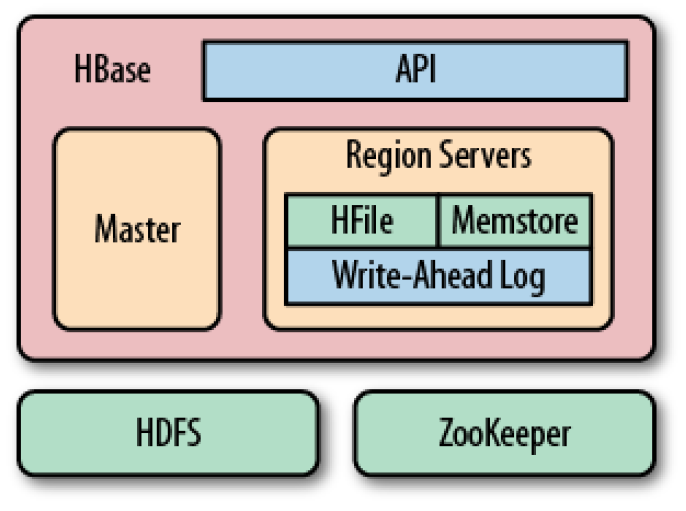
\includegraphics[width=0.5\linewidth]{images/hbasearch.png}
		\end{figure}
		\subsubsection{Overview}
		The master node (HMaster) assigns regions (key space) to region servers using zookeeper, handles load balancing (ZooKeeper) and holds metadata and schema.\newline
		Region servers handle reads and writes, the WAL and HFiles, and region splitting.
		\subsubsection{B+ Trees vs LSM Trees}
		B+ Trees use dynamic, multi-level indexes for efficient insertion, lookup and deletion. Frequent updates may imbalance the tree and a costly re-organization is required.\newline
		They support large scans, no costly tree-traversal algorithm is needed.\newline
		Updated and deletes are done at disk seek rates, rather than transfer rates.\newline
		\newline
		LSM Trees work at disk transfer rate and scale better to huge amounts of data. They guarantee a consistent insert rate (transforming random writes into sequential ones).\newline
		Reads are independent from writes. The optimized data layout offers predictable boundaries on disk seeks.
		\begin{figure}[H]
			\centering
			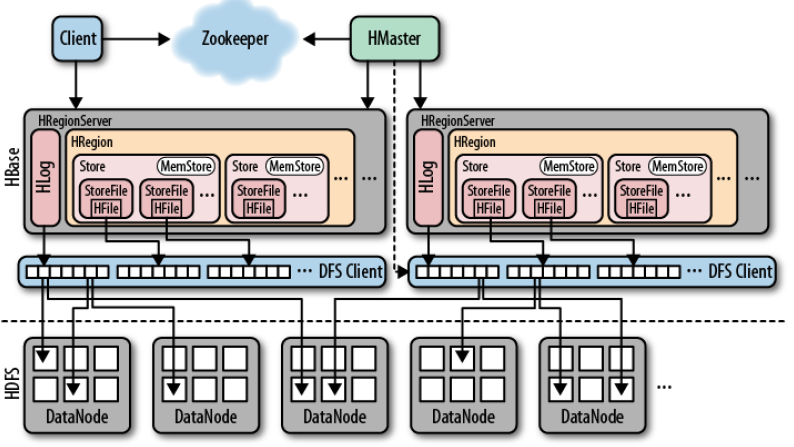
\includegraphics[width=0.7\linewidth]{images/hbasestorage.png}
		\end{figure}
	\subsection{Key Design}
		HBase has two fundamental key structures> row key and column key, they store meaningful data and their sorting is important.
		\subsubsection{Logical and physical layout of a table}
			 The main unit of separation within a table is the column family. Differently than the traditional column-based DBs, columns are not used to separate data, cells are stored logically in a table format and rows are stored as linear sets of cells.\newline
			 In the logical layout the table consist of rows and columns, this layout is folded so that the cells of each row are stored one ofter the other but each column family is stored separately (cells of one family reside on an individual HFile). HBase does not store unset cells.
			 Multiple versions of the same cell are stored consecutively, together with the timestamp, they are ordered in descending order so that the newest value is the first.
			 \begin{figure}[H]
			 	\centering
			 	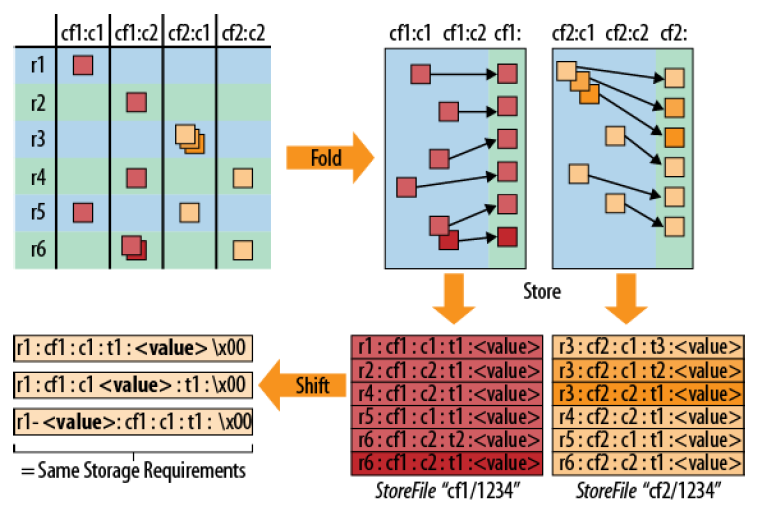
\includegraphics[width=0.65\linewidth]{images/hbaselayout.png}
			 \end{figure}
			 From the physical layout it is possible to select data by row-key from the different StoreFiles, this reduces the amount of data to scan for a row or a range of rows. When selcting data by row and column key, the system focuses on an individual storage. If the column qualifier is used, the system uses exact lookups, including filters to omit useless data.\newline
			 \newline
			 Given this query granularity, it is recommended to have tall-narrow tables with few columns and many rows.\newline
			 When missing the column key, the partial key scan allows to scan all the values for a given row key.
		\subsubsection{Time Series Data}
			If we use the timestamp as row key for time series data, HBase will store all rows sorted in a distinct range in regions with specific start and stop regions. Because of the sequential monotonously increasing nature of the data, they will all be written to the same region (hence to the same server).\newline
			In order to avoid this scenario different solutions exist:
			\begin{itemize}
				\item \textbf{Salting} had a non sequential prefix (hash) to the row key. Data access need to be fanned out across many servers but we can use multiple threads to read to improve I/O performance.
				\item \textbf{Promotion} move the timestamp field (field swap) or prefix it with another field (promotion), the sequential timestamp passes in second place. This way you can only access data (especially time ranges) for a given swapped or promoted field (but this could be a feature) but, as a pro, you achieve load balancing.
				\item \textbf{Randomization} hash the timestamp and use it has a key (MD5), this gives a random distribution of the row keys across all available region servers. It is less ideal for range scans but, since you can re-hash the timestamp, this solution is good for random access.
			\end{itemize}
			\begin{figure}[H]
				\centering
				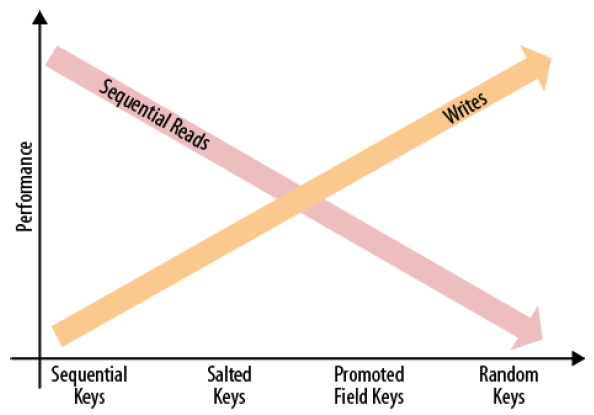
\includegraphics[width=0.46\linewidth]{images/timeseries.png}
			\end{figure}
	
\section{Apache Cassandra}
	\subsection{Overview}
	Cassandra is a distributed key-value that uses a column oriented model. There are no masters, every node can be whatever he wants, there is no single point of failure.\newline
	It has tunable consistency: it is often eventually consistent (AP) but it can shift to CP.\newline
	\newline
	It combines the HBase data model (one key per row, column and column families) and the Dynamo architecture (consistent hashing, anti-entropy replication and gossip-based membership).
	\subsection{Data Partitioning}
	The partitioning strategy can be changed on the fly but it needs to be chosen carefully because all data needs to be reshuffled.
		\subsubsection{Random Partitioner}
		It uses hash-based identifiers for keys and storage nodes (supports virtual nodes). Load monitoring (per ring) is added to consistent hashing: lightly loaded nodes are moved on the ring to alleviate heavily loaded ones. Deterministic choices are made about load balancing: divide the ring evenly with reference to the number of nodes.\newline
		Node addition and suppression requires re-balancing the cluster if there are no virtual nodes.
		\subsubsection{ByteOrdered Partitioner}
		It supports \textbf{range queries}, ensures row keys to be stored in sorted order. There is still a ring but keys are ordered lexicographically along the ring by their value. It might be bad for load balancing but range scan can be obtained by using column family indexes.
	\subsection{Data Replication}
	Replication is asynchronous, it walks down the ring, chooses \textit{N - 1} successor nodes as replicas and builds a preference list.\newline
	There are two main replication strategies, with \textbf{Simple strategy} the main replica is on the node responsible for a key and the additional ones are placed on the successor nodes. \textbf{NetworkTopology Strategy} allows better performance because of the knowledge of the datacenter layout (rack aware like HDFS). This requires Snitches  and optionally Zookeeper. Replica placement is independent in each datacenter.\newline
	There may be a potentially unbalanced load across the datacenter.
	\subsection{Data Model}
	The data model is column based. Each column stores counters containing timestamps. There could be expiring columns with a specified TTL. It also uses super columns to group multiple columns.
	\subsection{Read/Write Operations}
	Proxy nodes handle the interactions between the client and Cassandra, they determine the replicas for a given key and route the request to any replica.
		\subsubsection{Write request}
		The proxy node forwards the write request to all \textit{N} replicas but wait only for \textit{W} acks.\newline
		First the write is written in the \textbf{commit log}, then to an in-memory data structure (\textbf{memtable}) and finally writes are batched and periodically flushed to a persistent data structure: the \textbf{Sorted String Table}, SST (equivalent of HFile).\newline
		The memtables are organized in sorted order by row key and flushed to SSTables sequentially.\newline
		A single row can be stored in many SStables, at read time rows must be combined from all SSTables to produce the requested data.\newline
		To optimize this process \textbf{Bloom Filters} are used, they have \textit{k} hash functions hashing in the same \textit{m}-bit space. They are used when combining row data from multiple sources, they check if a requested row key exists in the SSTables before doing any disk seeks.
		\subsubsection{Read request}
		They use a similar mechanism to Dynamo if inconsistent replicas are detected, the number of replicas contacted upon a request depends on the consistency level.\newline
		When a node receives a read request, the row must be combined from all SSTables in that node and the data still stored in memtables.\newline
		To achieve higher performance Bloom Filters and the row level column index are used.
	\subsection{Consistency}
	Consistency is tunable and \textit{W} and \textit{R} are used as in Dynamo, but \textit{W + R $>$ N} is not mandatory.
		\subsubsection{Level ONE}
		\textit{W = 1}, one replica must write to commit log and memtable.\newline
		\textit{R = 1}, it returns a response from the closest replica (determined by the snitch).
		\subsubsection{Level QUORUM}
		\textit{W = floor(N/2 + 1)} and \textit{R = floor(N/2 + 1)}, it returns the record with the most recent timestamp.\newline
		If \textbf{LOCAL\_QUORUM}, it is restricted to a local data center.
		If \textbf{EACH\_QUORUM}, it must be satisfied across datacenters.
		\subsubsection{Level ALL}
		\textit{W = N} and \textit{R = N}.
		\subsubsection{Level ANY}
		Uses hinted handoff mechanism to add additional consistency for writes, it allows write to complete even if all \textit{N} replicas are down.
		\subsubsection{Level SERIAL}
		Lightweight transactions are used, they are a simple mechanism at the single key level, there is no support for multi-key transactions.
	
		

\chapter{Coordinating Distributed Systems}

\section{Two-phase commit}
	Two-phase commit is the simplest consensus protocol. It works in two phases: during phase 1 one coordinator node \textit{C} suggests a value to the other nodes and gather the responses; in phase 2, if all nodes agree, \textit{C} sends a commit command, abort otherwise.\newline
	\begin{figure}[H]
		\centering
		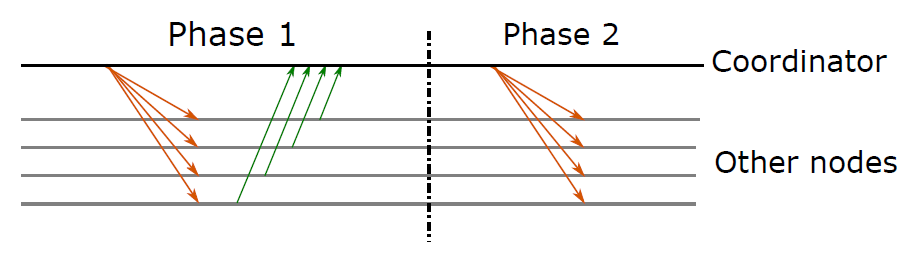
\includegraphics[width=0.8\linewidth]{images/twophasecommit.png}
	\end{figure}
	This protocol cannot make progress if there are simple failures. If \textit{C} fails in phase 1, it has to abort and retry, if it fails in phase 2, it has to replay the outcome (commit/abort). In both cases the outcome is uncertain until \textit{C} restarts.\newline
	If just one of the other nodes crashes, is slow or unreachable, the value cannot be committed.
	
\section{Paxos}
	Paxos uses state-machine replication, state machines ae fully deterministic: committed operations are executed in the same order by all state machines in the cluster.\newline
	The problem of Paxos is it is too complex and difficult to implement, there there are 5 different roles, the leader can work with a subset of the available nodes (quorum), there can be multiple proposals in the same round..
	\subsection{A simplified Paxos round}
		\subsubsection{Phase 1}
		A node in the cluster self-appoints as leader and chooses a new ballot ID. It sends a ballot proposal to the other nodes and they return the highest ballot ID they know (they can include their proposal for the value). If a majority responds with the proposed ID, the protocol can proceed.
		\begin{figure}[H]
			\centering
			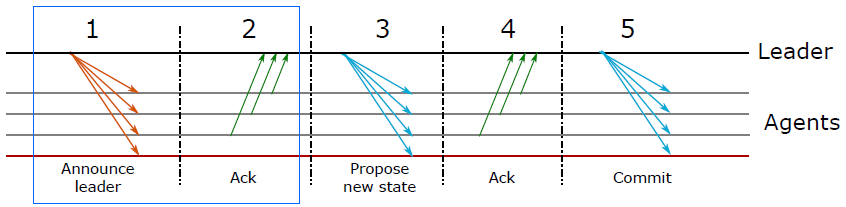
\includegraphics[width=0.8\linewidth]{images/paxos.png}
		\end{figure}
		\subsubsection{Phase 2}
		The leader resolves any conflicting proposal for the value and proposes it to the nodes. The nodes answer to the leader and, if a majority accepts the new value, it is final for this round, otherwise a new round must be started.

\section{Raft}
	\subsection{Overview}
	Raft implements distributed state machines too, it maintains a distributed log containing state machine commands.\newline
	The elected \textit{leader} handles all communications with the clients (no comms otherwise) and has the control on which entries are committed to the log.\newline
	All nodes are known in advance, the other nodes are passive replicators, periodic heartbeats are used to check if nodes are alive.\newline
	Snapshotting is used to keep the log size limited. 
	\subsection{Elections}
		At any given time each node is either a \textbf{leader}, a \textbf{follower} or a \textbf{candidate}.\newline
		Time is divided into terms, each identified by a monotonically increasing ID. All messages are labelled with a \textbf{term ID} used to identify obsolete information.\newline
		\newline
		Each node has a random timer, the \textbf{election timeout}. If anode does not receive any leader heartbeat before the timeout, it starts an election: it increments the term ID, becomes a candidate and votes for itself.\newline
		If it receives a majority of votes then it becomes a leader, if it receives a message from another leader, then it becomes a follower. No one wins before the election timeout expires again.
		\subsubsection{Election properties}
			\textbf{Safety}: there is at most one winner per term. Each voter votes only once per term and there cannot be two majorities in the same term.\newline
			\textbf{Liveness}: a leader will eventually be elected, the randomness of the timeout guarantees there will be different candidates at different times.\newline
			Faults causing new terms happen rarely compared to a second-lasting election.
	\subsection{Operation}
		Clients send commands to the current leader\newline
		The leader logs a new (uncommitted) entry\newline
		The leader sends the new entry to all nodes in the next heartbeat\newline
		Once a majority answers, the leader commits the new entry\newline
		The leader answers the client\newline
		The leader asks all nodes to commit the entry in the next heartbeat\newline
		The nodes commit the entry in their logs.
	\subsection{Failures Handling}
		\subsubsection{Leader failure}
			After the election timeout, a new leader is elected.\newline
			It will restart as a follower and set its internal term ID according to the first heartbeat message he receives. The leader will send it the missing log entries.\newline
			The client will never receive the commit ack and uncommitted entries in the followers will eventually be overwritten by the new leader.
		\subsubsection{Follower failure}
			Nothing happens and the restart process is the same as if it was leader.
		\subsubsection{50/50 vote (split majority)}
			No leader is elected, timeout expires and therefore there is a new term and a new election.\newline
			Fortunately, there is a really low probability for this to happen.
		\subsubsection{Network partition}
			The majority rule ensures only half of the partition commits new entries.\newline
			The biggest partition will elect a leader, incrementing the term ID, while the smaller one will be unable to do so (no majority).\newline
			When the partition is healed, the minority partition will receive heartbeats with a bigger term OD, uncommitted logs will be overwritten and the leader in the minority partition (if any) will immediately step down.
\section{Zoe and ZooKeeper}
	\subsection{Overview}
		When building a distributed system, one can either build his own coordination primitives (error-prone approach) or use an external coordination system, this will add external dependencies but a tested and well known system will be used.\newline
		\newline
		ZooKeeper objectives are: a simple interface, a highly available architecture and to provide common services needed by distributed systems (configuration, group management, naming, presence protocols, synchronization).
	\subsection{Architecture}
		ZooKeeper itself is distributed, for performance and fault tolerance. Clients can talk to any server but all update operation are handled by an elected leader.\newline
		Data is kept in memory for performance while snapshots and transaction logs are on persistent storage.\newline
		\newline
		ZooKeeper is AP by default: reads return local chached data\footnote{ZooKeeper writes are always synchronized through the leader.}, but the client may use the sync command to flush all caches, this will make ZooKeeper CP but there wil be a performance penalty.
		\subsubsection{ZAB}
		ZAB is the consensus protocol used by ZooKeeper (does not use state machines). It totally orders write requests using a majority of ZooKeeper processes, the leader sequences the requests and invokes ZAB atomic broadcast. Strictly ordered state updates are applied by non-leaders.\newline
		Developers focused on \textbf{strong ordering guarantees for all operations}.\newline
		\newline
		The data model is made of a hierarchical namespace (like a file system) where each node, called \textit{znode}, can contain data and have children.\newline
		Znodes can be:
		\begin{itemize}
			\item \textbf{Regular}, created and destroyed by the client
			\item \textbf{Ephemeral}, created by the client, deleted by ZooKeeper if he disconnects
			\item \textbf{Sequential}, created by the client, but the name is generated by ZooKeeper using a counter
			\item \textbf{Ephemeral + Sequential}
		\end{itemize}
		Znodes have version counters that are updated each time their content changes. A client can set a \textbf{watch} on a znode so that ZooKeeper will call him back when the data changes or a znode i created or destroyed. Watches are very useful to implement locks and leader elections with good performance.
	\subsection{Implementation}
		\subsubsection{Consensus}
		A number of processes need to agree on a value, each one proposes with \textit{create(PATH, my\_value, SEQUENTIAL)} and then each process decides:\newline
		\textit{C = getChildren(PATH)}\newline
		\textit{select znode z in C with smallest sequence suffix}\newline
		\textit{agreed\_value = getData(PATH + z)}		\subsubsection{Configuration Management}
		A number of processes need to access a common configuration which can change dynamically.\newline
		They put a watch on the configuration path and update configuration when notified of a change.
		\subsubsection{Group Membership}
		A number of processes provide the same service (load balancing), we need to leverage the ephemeral nodes.\newline
		Each process join the group so a watch is used to get notified about membership changes.
\backmatter
% bibliography, glossary and index would go here.

\end{document}